% Options for packages loaded elsewhere
% !TeX program = xelatex
\PassOptionsToPackage{unicode}{hyperref}
\PassOptionsToPackage{hyphens}{url}
\documentclass[a4paper,11pt]{article}
\hfuzz=10pt
% ------------------------------------------------------------
% XeLaTeX + Unicode fonts
% ------------------------------------------------------------
\usepackage{fontspec}
\usepackage{unicode-math}
\usepackage{polyglossia}
\setdefaultlanguage{english}
% Code listings and flexible tables
\usepackage{listings}
\usepackage{tabularx}

% --- TEXT + MATH FONTS (FULL UNICODE COVERAGE) ---
\setmainfont{Libertinus Serif}
\setmathfont{Libertinus Math}

% sensible defaults
\defaultfontfeatures{Scale=MatchLowercase, Ligatures=TeX}
\defaultfontfeatures[\rmfamily]{Ligatures=TeX, Scale=1}

% ------------------------------------------------------------
% Bibliography
% ------------------------------------------------------------
\usepackage{csquotes}
\usepackage[backend=biber,style=numeric]{biblatex}
\addbibresource{references.bib}

% ------------------------------------------------------------
% General layout / math / colours
% ------------------------------------------------------------
\usepackage{xcolor}
\usepackage{amsmath}

\lstdefinestyle{codeblock}{%
  language={[Sharp]C},
  basicstyle=\ttfamily\scriptsize,
  backgroundcolor=\color{black!5},
  frame=single,
  float,
  floatplacement=htbp,
  columns=fullflexible,
  keepspaces=true,
  breaklines=true,
  tabsize=2,
  showstringspaces=false,
  upquote=true
}

\lstdefinestyle{datadump}{%
  basicstyle=\ttfamily\scriptsize,
  backgroundcolor=\color{black!3},
  frame=single,
  float,
  floatplacement=htbp,
  columns=fullflexible,
  keepspaces=true,
  breaklines=true,
  tabsize=2,
  showstringspaces=false,
  upquote=true
}

\lstdefinestyle{datadumpnofloat}{%
  basicstyle=\ttfamily\scriptsize,
  backgroundcolor=\color{black!3},
  frame=single,
  columns=fullflexible,
  keepspaces=true,
  breaklines=true,
  tabsize=2,
  showstringspaces=false,
  upquote=true
}


\lstnewenvironment{diagram}{%
  \lstset{
    style=codeblock,
    keywordstyle={}
  }%
}{}

\lstnewenvironment{datadump}{%
  \lstset{
    style=datadump
  }%
}{}

\lstnewenvironment{datadumpnofloat}{%
  \lstset{
    style=datadumpnofloat
  }%
}{}

\unimathsetup{
  math-style=TeX,
  bold-style=TeX
}

% Use upquote if available
\IfFileExists{upquote.sty}{\usepackage{upquote}}{}

% Microtypography
\IfFileExists{microtype.sty}{%
  \usepackage[]{microtype}
  \UseMicrotypeSet[protrusion]{basicmath}%
}{}

% ------------------------------------------------------------
% Paragraph spacing (Pandoc-style)
% ------------------------------------------------------------
\makeatletter
\@ifundefined{KOMAClassName}{%
  \IfFileExists{parskip.sty}{\usepackage{parskip}}{%
    \setlength{\parindent}{0pt}
    \setlength{\parskip}{6pt plus 2pt minus 1pt}%
  }%
}{\KOMAoptions{parskip=half}}
\makeatother

% ------------------------------------------------------------
% Tables & helpers
% ------------------------------------------------------------
\usepackage{longtable,booktabs,array}
\usepackage{calc}
\newcommand{\real}[1]{#1}
\usepackage{etoolbox}
\makeatletter
\patchcmd\longtable{\par}{\if@noskipsec\mbox{}\fi\par}{}{}
\makeatother

\IfFileExists{footnotehyper.sty}{\usepackage{footnotehyper}}{\usepackage{footnote}}
\makesavenoteenv{longtable}

% ------------------------------------------------------------
% Graphics & Pandoc image scaler
% ------------------------------------------------------------
\usepackage{graphicx}
\makeatletter
\newsavebox\pandoc@box
\newcommand*\pandocbounded[1]{%
  \sbox\pandoc@box{#1}%
  \Gscale@div\@tempa{\textheight}{\dimexpr\ht\pandoc@box+\dp\pandoc@box\relax}%
  \Gscale@div\@tempb{\linewidth}{\wd\pandoc@box}%
  \ifdim\@tempb\p@<\@tempa\p@\let\@tempa\@tempb\fi%
  \ifdim\@tempa\p@<\p@\scalebox{\@tempa}{\usebox\pandoc@box}%
  \else\usebox\pandoc@box%
  \fi%
}
\def\fps@figure{htbp}
\makeatother

% ------------------------------------------------------------
% Code-breaking for long identifiers
% ------------------------------------------------------------
\newcommand{\codebreak}[1]{\texttt{\begingroup\hyphenchar\font=`\- #1\endgroup}}

\newcommand{\PVGet}{\codebreak{PositronicVariable<T>.GetCurrentQBit()}}
\newcommand{\ListString}{\codebreak{List<string>}}
\newcommand{\Assign}{\codebreak{Assign()}}
\newcommand{\ConstrainEqual}{\codebreak{ConstrainEqual()}}
\newcommand{\QExpr}{\codebreak{QExpr}}


% ------------------------------------------------------------
% Line-breaking / lists (Pandoc)
% ------------------------------------------------------------
\setlength{\emergencystretch}{3em}
\providecommand{\tightlist}{%
  \setlength{\itemsep}{0pt}\setlength{\parskip}{0pt}}

% ------------------------------------------------------------
% URLs, bookmarks, links
% ------------------------------------------------------------
\IfFileExists{xurl.sty}{\usepackage{xurl}}{}
\usepackage{hyperref}
\usepackage{bookmark}
\urlstyle{same}
\hypersetup{
  pdftitle={QuantumSuperposition and PositronicVariables},
  hidelinks,
  pdfcreator={LaTeX via pandoc},
}

% Polyglossia injects language metadata into caption labels via \@caption.
% In this monolingual document, restoring the original caption writer avoids
% malformed aux entries on clean rebuilds.
\ExplSyntaxOn
\AddToHook{begindocument/end}{
  \cs_if_exist:cT { __xpg_save_caption:n }
    {
      \cs_set_eq:cc { @caption } { __xpg_save_caption:n }
    }
}
\ExplSyntaxOff

% ------------------------------------------------------------
% Title / Subtitle
% ------------------------------------------------------------
\title{QuantumSuperposition and PositronicVariables}
\author{Paul Hutchinson\\Findon Software\\
\texttt{ORCID: 0009-0009-8578-2649}}
\date{}
\makeatletter
\providecommand{\subtitle}[1]{%
  \apptocmd{\@title}{\par {\large #1 \par}}{}{}
}
\makeatother
\subtitle{Strongly-Typed Multiverse Programming, Quantum-Inspired Circuits, and Temporal Self-Consistency for .NET}
\begin{document}

\maketitle
\tableofcontents
\bigskip

\begin{abstract}
\sloppy
This paper presents \textbf{QuantumSuperposition} and \textbf{PositronicVariables}, 
two interlinked .NET libraries for modelling uncertainty, quantum-style superposition, 
and time-looped convergence in ordinary C\# code. QuantumSuperposition provides 
(1) a \textbf{generic superposition engine} in the form of \texttt{QuBit<T>} and 
\texttt{Eigenstates<T>} with complex amplitudes, arithmetic, LINQ integration 
and non-destructive sampling, and 
(2) a \textbf{physics-flavoured quantum layer} with multi-qubit QuantumSystem, 
entanglement management, gate catalogues, canonical states, and bundled 
implementations of the Quantum Fourier Transform (QFT) and Grover's search 
algorithm.\parencite{Pau25}

PositronicVariables builds on the same superposition semantics to model 
\textbf{reversible temporal logic}: variables that can participate in feedback loops, 
roll their state backwards and forwards through hypothetical timelines, and converge 
to a consistent fixed point (or, in pathological cases, a politely documented paradox).

We additionally use David Deutsch's self-consistency condition for quantum
systems interacting with closed timelike curves as a software-design analogy for
PositronicVariables: when a value depends on the context it helps create, the
runtime searches for states that can survive the loop, including stable plural
outcomes where no single classical answer is adequate.\parencite{Deutsch91CTC}

The resulting ecosystem lets .NET developers treat “maybe” and “many possible futures” 
as first-class values while still enjoying static typing, IDE autocompletion and the 
reassuring hum of the garbage collector. We describe the design and semantics of both 
layers, motivate their use as teaching and experimentation tools, and compare them to 
existing quantum SDKs and probabilistic programming languages. Our guiding design 
principle is simple: \textbf{make the multiverse feel like idiomatic C\#}, with just 
enough weirdness to be fun but not enough to summon an actual physicist.\footnote{
No actual cats were placed in superposition during this work; only unit tests. All 
boxes are purely metaphorical, and any resemblance to real laboratory apparatus, 
living or dead, is strictly coincidental.
}
\fussy
\end{abstract}

\section{Introduction}

Classical programs are famously decisive: a variable typically has one value, at one time, in one universe. This is convenient for compilers but an awkward fit for many real-world problems where we genuinely care about \textbf{sets of possibilities}, \textbf{probabilities}, and ``what if'' scenarios that feed back into themselves.

In parallel, quantum computing has made ``superposition'' and ``entanglement'' part of the mainstream programming vocabulary, at least for values of ``mainstream'' that include people who read arXiv for fun. A rich ecosystem of quantum SDKs such as Qiskit~\parencite{pyp25}, circuit DSLs such as Quipper~\parencite{Green13Quipper}, and \textbf{Q\#}~\parencite{Mic25,Heim18QSharp} targets hardware and gate-level simulation. These tools are powerful, but they are often overkill when you simply want to:

\begin{itemize}
\item
Reason about many candidate values in parallel,
\item
Model probabilistic logic directly in a typed language, or
\item
Build small quantum-inspired toys that run in a unit test rather than in a dilution fridge.
\end{itemize}

At the same time, probabilistic programming languages like \textbf{Pyro}~\parencite{Goo19} and \textbf{WebPPL}~\parencite{Goodman14WebPPL} show that first-class uncertainty can be deeply integrated into a host language. Long before ``quantum machine learning'' became a conference track, \textbf{Damian Conway's Quantum::Superpositions module}\parencite{Dam25} for Perl demonstrated that scalar variables could cheerfully pretend to be superposed sets of values.

In this work, we try to bring those ideas - superposed values, quantum-style circuits, and convergent time loops - into modern .NET in a way that is:

\begin{enumerate}
\def\labelenumi{\arabic{enumi}.}
\item
\textbf{Strongly typed} (because if the compiler is not judging you, who will?),
\item
\textbf{Developer-friendly} (LINQ, NuGet, unit tests, the usual comforts), and
\item
\textbf{A fun read} (within the limits of arXiv and your sense of humour).
\end{enumerate}

\subsection{Self-consistency as a software problem}

In 1991, Deutsch proposed a treatment of quantum systems interacting with closed
timelike curves in which the chronology-violating part of the system must satisfy
a self-consistency condition.\parencite{Deutsch91CTC} Informally, if a system
meets its own past, the admissible states are the ones that can survive that loop
without contradiction. When no single pure state can do the job, the formalism may
settle on a mixed state over self-consistent possibilities.

This paper does not claim to simulate physical closed timelike curves. Instead, we
use Deutsch's move as a useful software-design lens. Ordinary programs increasingly
encounter analogous structures: cyclic dependencies, feedback graphs, self-referential
constraints, reactive systems, bidirectional state, reversible computation, and values
whose outputs are also part of their inputs. Once a computation has that shape, the
question is no longer merely ``what happens next?'' but ``what state can exist at all
without contradicting the loop?''

The central thesis of this framing is that software systems already embody different
answers to that question. Some reject inconsistent loops, some require the programmer
to tie the knot correctly, some search for satisfying assignments, some infer plausible
histories, and some prevent disagreement by construction. PositronicVariables takes a
different position: let the loop run, watch what stabilises, and expose the surviving
state or support as ordinary C\# data.

\paragraph{Grover search case study.}

A concrete two-qubit and three-qubit worked example, with empirical success probabilities, is given in Section~\ref{sec:grover-small-n}.
\subsection{Contributions}

This is a \textbf{system / library} paper: our contributions are about design, semantics and experience rather than new asymptotic bounds or formal theorems. Concretely, this work contributes:

\begin{itemize}
\item
\textbf{A design and semantics for a generic superposition type in C\#.}
We introduce QuBit\textless T\textgreater{} and Eigenstates\textless T\textgreater{} as a strongly typed model of ``one variable, many possible values'', with complex amplitudes, arithmetic, comparisons, LINQ integration, and reproducible collapse semantics.
Our model of typed superposition values parallels earlier work on quantum circuit DSLs such as Quipper~\parencite{Green13Quipper}, though our focus differs in targeting classical execution with multiverse-style semantics rather than hardware-level quantum control.
\item
\textbf{A minimal gate-level simulator with educational algorithms.}
The QuantumSystem / QuantumGate / QuantumAlgorithms layer implements a small, linear-algebra state-vector simulator with entanglement tracking, partial observation, gate scheduling, and textbook implementations of QFT and Grover search designed for classroom- and unit-test-scale examples.
\item
\textbf{A temporal convergence model with STM for ``multiverse timelines''.}
PositronicVariables provides a higher-level framework in which feedback loops over superposed values are resolved by a single-writer, STM-style convergence engine that computes fixed points over \emph{superpositions} rather than scalars, with explicit telemetry and replay.
\item
\textbf{A fixed-point view of temporal paradoxes and an empirical experience report.}
We treat paradoxical constraints as fixed points over superpositions and show how the runtime computes and exposes these, then report on how the combined abstractions behave in practice as teaching tools and as a playground for quantum-inspired algorithms (lightweight, honest, and slightly self-deprecating).
\item
\textbf{A comparative framing of cyclic consistency in software.}
We position PositronicVariables against existing software responses to self-reference:
time-travel languages, bidirectional state, probabilistic programming, constraint and
logic systems, reversible languages, and quantum data-structure or decision-diagram
tooling. This is not presented as a new theorem, but as a design-space map for how
software handles loops that are allowed to talk back.
\end{itemize}

Throughout, we emphasise how to express ``multiverse thinking'' in everyday C\#. Here, ``multiverse'' simply means reasoning about many possible program states at once, not a commitment to any particular physical interpretation of quantum mechanics and not an attempt to force developers to abandon their IDE, their existing build pipeline, or their deep emotional attachment to IEnumerable\textless T\textgreater{}.

\section{Background}

\subsection{Quantum superposition in one paragraph (and a bit)}

\newcommand{\ket}[1]{\lvert #1 \rangle}

In quantum mechanics, \textbf{superposition} means that a system can be in a linear combination of basis states at once, with complex amplitudes that determine measurement probabilities. A single qubit lives in a state
\[
\ket{\psi} = \alpha \ket{0} + \beta \ket{1},
\]
subject to $|\alpha|^2 + |\beta|^2 = 1$ \parencite{Nie10}.

Measurement turns this graceful linear-algebra object into one definite outcome, with probability given by the squared magnitude of the corresponding amplitude. Phase differences between amplitudes, invisible to classical eyes, become crucial when gates interfere constructively or destructively.

QuantumSuperposition's physics layer is a conventional state-vector simulator that implements exactly this story: complex amplitudes, unitary matrices, and measurement as sampling with $\lvert \mathrm{amp} \rvert^{2}$ probabilities. The generic superposition layer generalises the idea: instead of basis states $\ket{0}$ and $\ket{1}$, we allow arbitrary values of type~T, but keep the ``weighted possibilities'' intuition.

\subsection{Closed timelike curves and self-consistency}

Deutsch's closed-timelike-curve model can be read, at a high level, as a fixed-point
condition on states. A chronology-respecting system interacts with a chronology-violating
system, and the latter must emerge from the interaction in a state compatible with
the state that entered it.\parencite{Deutsch91CTC} The important software analogy is
not the spacetime geometry, but the discipline: a loop is admissible only when the
state around the loop is self-consistent.

There is an important distinction here. In Deutsch's physical setting, the formal
objects are density matrices and mixed quantum states. In QuantumSuperposition and
PositronicVariables, the objects exposed to the programmer are \texttt{QuBit<T>}
instances, weighted eigenstates, supports, timelines, and convergence reports. We
therefore use ``Deutsch-style'' or ``CTC-style'' only to mean ``self-consistency over
a loop'', not ``a faithful density-matrix simulation of a real time machine''.

\subsection{Related ecosystems and cyclic consistency}

Two kinds of tools are particularly relevant:

\begin{itemize}
\item
  	\textbf{Quantum SDKs} such as Qiskit and Q\# expose quantum circuits, gates and backends (simulators or hardware). They target realistic devices and resource estimation.\parencite{pyp25,Heim18QSharp}
\item
  	\textbf{Probabilistic programming languages} such as Pyro and WebPPL treat probability distributions as first-class objects and provide inference algorithms to match.\parencite{Goo19,Goodman14WebPPL}
\end{itemize}

Hosted quantum circuit DSLs such as Quipper~\parencite{Green13Quipper} demonstrate that one can treat circuits as first-class values inside a classical host language; our generic superposition layer plays a similar role for typed superposition values, while remaining purely classical.

QuantumSuperposition deliberately sits \textbf{between} these camps: it is not tied to any quantum hardware platform and does not attempt general Bayesian inference. Instead, it gives C\# developers a compact set of abstractions that:

\begin{itemize}
\item
  Feel natural in the .NET ecosystem,
\item
  Are simple enough to understand from the source code,
\item
  Yet are rich enough to play with genuine quantum algorithms like QFT and Grover search.
\end{itemize}

On the language-design side, Conway's \textbf{Quantum::Superpositions} in Perl is a clear ancestor: it introduced ``superpositions stored in a scalar variable'' and overloaded operators such as any and all to act over many values at once.\parencite{Dam25} QuantumSuperposition updates the idea for a strongly typed, generics-heavy world and extends it with explicit linear-algebra semantics and a temporal convergence layer.

\subsubsection{Attitudes to paradox in existing software}

Seen through the self-consistency lens, these systems are not just unrelated
curiosities. They are different attitudes to the same family of problems: values that
depend on each other non-sequentially, computations whose outputs constrain their
inputs, and loops where the runtime must decide what counts as an admissible state.

\begingroup
\small
\setlength{\LTleft}{0pt}
\setlength{\LTright}{0pt}
\begin{longtable}{@{}
  >{\raggedright\arraybackslash}p{0.16\linewidth}
  >{\raggedright\arraybackslash}p{0.18\linewidth}
  >{\raggedright\arraybackslash}p{0.30\linewidth}
  >{\raggedright\arraybackslash}p{0.28\linewidth}
@{}}
  \caption{Different software attitudes to cyclic consistency and self-reference}\label{tab:attitudes-to-paradox}\\
  \toprule
  \textbf{Approach} &
  \textbf{Attitude to loops} &
  \textbf{Typical behaviour} &
  \textbf{Contrast with PositronicVariables} \\
  \midrule
  \endfirsthead
  \toprule
  \textbf{Approach} &
  \textbf{Attitude to loops} &
  \textbf{Typical behaviour} &
  \textbf{Contrast with PositronicVariables} \\
  \midrule
  \endhead
    Mariposa &
    Refusal by runtime guard &
    Provides explicit time-travel primitives, but rejects conflicting or invalid
    temporal edits.\parencite{MariposaGitHub} &
    PositronicVariables does not merely reject disagreement; it tries to compute
    the stable support that survives it. \\

    Tardis &
    Elegant knot-tying &
    Lets state travel both forwards and backwards through a Haskell computation,
    assuming the programmer has arranged the knot coherently.\parencite{TardisHackage} &
    PositronicVariables treats the knot as something the convergence engine may
    have to negotiate. \\

    Probabilistic programming &
    Bayesian filtering &
    Languages such as Church, WebPPL, Pyro, and Infer.NET condition possible
    histories on observations and weight the survivors.\parencite{Church2008,Goodman14WebPPL,Goo19,Mic251} &
    PositronicVariables is not a general inference engine; it reports stable
    program-state supports directly. \\

    Constraint, logic, and propagator systems &
    Search and propagation &
    miniKanren, truth-maintenance systems, and propagator networks search for,
    propagate, or explain mutually compatible assignments.\parencite{MiniKanren,Doyle79TMS,RadulSussman09} &
    PositronicVariables exposes the surviving support as a typed value inside
    ordinary imperative C\# code. \\

    Reversible languages &
    Consistency by construction &
    Languages such as Janus and Sparcl make computations invertible or partially
    invertible, so disagreement is often avoided structurally.\parencite{YokoyamaGluck07Janus,MatsudaWang24Sparcl} &
    PositronicVariables allows more ordinary, non-invertible code to participate
    in cyclic convergence. \\

    Quantum data-structure and decision-diagram tools &
    Formal substrate &
    Tower and Q-Sylvan operate closer to quantum formalisms, reversible semantics,
    or decision-diagram representations.\parencite{YuanCarbin22Tower,BrandLaarman25QSylvan} &
    PositronicVariables aims to make stable plurality printable, inspectable,
    and usable by ordinary .NET developers. \\

    PositronicVariables &
    Stable plurality as data &
    Runs a convergence process over superposed timelines and returns either a
    fixed point, a stable support such as \texttt{any(-1, 1)}, or diagnostics. &
    This is the contribution developed in Sections~\ref{sec:pv-self-consistency}
    through~\ref{sec:positronic-case-studies}. \\
  \bottomrule
\end{longtable}
\endgroup

This comparison is intentionally pragmatic. Constraint systems and probabilistic
languages are deeper and more general in their own domains; reversible languages
provide stronger semantic guarantees; quantum simulators expose more faithful
linear-algebra machinery. The point is narrower: PositronicVariables occupies the
specific niche where cyclic ordinary-code relationships can stabilise to a plural
typed value rather than an exception, an external solver result, or an inferred
posterior distribution.

\subsection{Scope and non-goals}

Before we go further, several disclaimers:

\begin{itemize}
\item
  We are \textbf{not} building a high-precision physics simulator; double-precision complex numbers and reasonably sized state vectors are perfectly acceptable here.
\item
  We are \textbf{not} claiming quantum advantage; all code runs on vanilla CPUs and is fully classical.
\item
  We are \textbf{not} inventing a new foundational interpretation of quantum mechanics (although the library does have opinions about cats, collapse and what counts as ``observing'').
\item
  We are \textbf{not} claiming to simulate physical closed timelike curves. The Deutsch comparison is a conceptual and computational analogy about fixed points over loops, not a physics claim about spacetime or density matrices.
\end{itemize}

Instead, this work aims to provide:

\begin{enumerate}
\def\labelenumi{\arabic{enumi}.}
\item
  A testbed for quantum-inspired teaching and experimentation in C\#, and
\item
  A playful, yet technically coherent, way to reason about multiple possible values and timelines.
\end{enumerate}

\subsection{Intended audience}

This paper is written primarily for \textbf{practicing C\# / .NET developers} and \textbf{technically inclined readers} who are curious about quantum-style ideas but would prefer to explore them without leaving their IDE.

We assume basic familiarity with:
\begin{itemize}
\item modern C\# features (generics, LINQ, interfaces, basic async/await),
\item elementary linear algebra notation at the level of ``vectors, matrices, and inner products'',
\item the standard ``textbook'' quantum computing cast of characters: qubits, single- and two-qubit gates, simple circuits, and canonical algorithms such as the Quantum Fourier Transform (QFT) and Grover's search.
\end{itemize}

We \emph{do not} assume:
\begin{itemize}
\item prior experience with quantum SDKs, hardware backends, or noise models,
\item a background in functional programming, category theory, or denotational semantics,
\item enthusiasm for long, epsilon--delta proofs (there are no new theorems here).
\end{itemize}

This is explicitly a \textbf{system and library paper}, not a ``new theorem'' or ``new algorithm'' paper. The focus is on the design and semantics of the abstractions, their implementation in ordinary C\#, and an honest experience report on how they behave in practice as teaching tools and as a playground for quantum-inspired experiments.

\section{Design Goals}

Across both libraries we adopted five main design goals. In very compressed form,
they are: make superposition feel normal, keep the compiler on your side, be random
on purpose rather than by accident, report stable plurality honestly, and let the
jokes do some of the teaching.

\begin{enumerate}
\def\labelenumi{\arabic{enumi}.}

\item
\textbf{First-class superposition}\
Make ``one variable, many possible values'' feel as boringly normal as List\textless T\textgreater{}, while still exposing enough structure (weights, collapse, sampling) that the quantum metaphor is not just decorative. Superpositions should slot naturally into ordinary C\# code without demanding a new mental model for every line.

\item
\textbf{Type safety and IDE friendliness}\
Avoid ``stringly typed quantum'' in favour of generics, interfaces and C\#'s usual tooling: autocomplete, refactoring and static checks. Wherever possible, superposed values participate in familiar language features and library patterns so that most of the time developers are writing `ordinary'' C\# that just happens to be reasoning about many possibilities at once.

\item
\textbf{Determinism when you ask for it}\
Provide seeded random number generation, collapse replay and test-friendly APIs so that `quantum randomness'' does not become `my CI pipeline is haunted''. The same scenario can be re-run under a known seed, logged, debugged locally and then replayed in a test harness without surprises.~\parencite{Pau25}

\item
\textbf{Stable plurality rather than premature collapse}\
When a feedback loop stabilises on a support preserved by the loop as a whole,
the runtime should expose that plurality as a value rather than hiding it behind
an exception, an arbitrary tie-break, or an opaque inference procedure. A result
such as \texttt{any(1, 2)} is not a shrug; it is a compact report of what survived
the consistency process.

\item
\textbf{Humour as documentation strategy}\
Use light-hearted names, examples and comments to lower the barrier to entry. The aim is not to trivialise the ideas but to make it easier to keep reading once the abstractions get dense; if you are going to model entanglement and time loops, you might as well collect a few jokes along the way.

\end{enumerate}

\section{QuantumSuperposition: Generic Superposition Layer}

\subsection{Core abstractions: QuBit\textless T\textgreater{} and Eigenstates\textless T\textgreater{}}

At the heart of the generic layer are two types:

\begin{itemize}
\item
  QuBit\textless T\textgreater{} - a multiset of values of type T, each associated with a (complex) amplitude.
\item
  Eigenstates\textless T\textgreater{} - a view over ``original keys'' vs derived values; useful when transforms change outputs but you still want to track where they came from.
\end{itemize}

Conceptually, a QuBit\textless T\textgreater{} represents a superposition

\[
\sum_i \alpha_i \ket{v_i}
\]

where vᵢ : T and $\alpha_i$ : Complex. Internally, this is stored as a dictionary or similar mapping from values to amplitudes, with normalisation exposed via helpers.
From a language-design perspective this is close in spirit to circuit-DSL approaches such as Quipper~\parencite{Green13Quipper}: circuits there, and superposed values here, are treated as first-class objects in a classical host, but we deliberately avoid any dependence on quantum hardware or resource estimation.

Key operations include:

\begin{itemize}
\item
  Construction from a list of values (uniform amplitudes) or an explicit map of amplitudes.
\item
  \textbf{Normalisation}: rescaling amplitudes so that the sum of squared magnitudes equals 1.
\item
  \textbf{Collapse} via .Observe(), which samples a value according to \textbar $\alpha_i$\textbar² and records the outcome for optional replay.
\item
  \textbf{Sampling without commitment} via helpers such as SampleWeighted() and MostProbable().
\end{itemize}

The library's documentation describes this succinctly as ``variables living in several states at once, then collapsing when you finally make up your mind''-an accurate description of both qubits and many human decisions.~\parencite{Pau251}.

  \textbf{Example: tiny multiverse of integers}

\begin{lstlisting}[style=codeblock]
var qubit = new QuBit<int>(new[] { 1, 2, 3 });
var doubled = qubit.Select(x => x * 2);
var sample = doubled.SampleWeighted();
Console.WriteLine(sample);
\end{lstlisting}

\subsubsection{A tiny worked example: probability tables before and after Select}\label{tiny-select-example}

\footnote{Select maps eigenvalues and merges amplitudes when targets collide. Because the input
is normalized, the resulting probabilities are computed over the derived eigenstate distribution;
in injective cases the per-branch weights carry through; in non-injective cases merged weights
reflect the number and phases of contributing branches (See Tables~\ref{tab:select-double}--\ref{tab:select-merge}).}

To make the semantics slightly less hand-wavy, consider again the minimal multiverse of integers:

\begin{lstlisting}[style=codeblock]
var qubit = new QuBit<int>(new[] { 1, 2, 3 });
var doubled = qubit.Select(x => x * 2);
var sample = doubled.SampleWeighted();
Console.WriteLine(sample);
\end{lstlisting}

The constructor \texttt{new QuBit<int>(new[] \{ 1, 2, 3 \})} creates a uniform superposition of the three eigenstates 1, 2 and 3. Internally, each value gets the same complex amplitude; for a real-valued uniform superposition this is

α₁ = α₂ = α₃ = 1/√3

so that the total probability mass stays at 1.

The initial state appears in Table~\ref{tab:initial-superposition}:
\begin{table}[htbp]
  \centering
  \begin{tabular}{@{}
    >{\raggedright\arraybackslash}p{(\linewidth - 4\tabcolsep) * \real{0.3333}}
    >{\raggedright\arraybackslash}p{(\linewidth - 4\tabcolsep) * \real{0.3333}}
    >{\raggedright\arraybackslash}p{(\linewidth - 4\tabcolsep) * \real{0.3334}}@{}}
  	\toprule
  \begin{minipage}[b]{\linewidth}\raggedright
  Eigenstate (value)
  \end{minipage} & \begin{minipage}[b]{\linewidth}\raggedright
  Amplitude $\alpha_i$
  \end{minipage} & \begin{minipage}[b]{\linewidth}\raggedright
  Probability $|\alpha_i|^2$
  \end{minipage} \\
  \midrule
  1 & 1/√3 & 1/3 \\
  2 & 1/√3 & 1/3 \\
  3 & 1/√3 & 1/3 \\
  \bottomrule
  \end{tabular}
  \caption{Eigenstates and probabilities of the initial uniform superposition}
  \label{tab:initial-superposition}
\end{table}

If we were to call qubit.Observe() at this point, each of 1, 2 and 3 would be returned with probability 1/3 (modulo seeding and collapse configuration), and the qubit would then be marked as collapsed.\parencite{Pau255}

However, the call to Select(x =\textgreater{} x * 2) does not collapse the state. Instead, it lifts the pure function x ↦ 2x over the eigenstates, giving us a new superposition in which:

\begin{enumerate}
\def\labelenumi{\arabic{enumi}.}
\item
  each original value v becomes 2v, and
\item
  the amplitudes are carried across unchanged.
\end{enumerate}
\begin{table}[htbp]
  \centering
  \begin{tabular}{@{}
    >{\raggedright\arraybackslash}p{0.26\linewidth}
    >{\raggedright\arraybackslash}p{0.22\linewidth}
    >{\raggedright\arraybackslash}p{0.26\linewidth}
    >{\raggedright\arraybackslash}p{0.26\linewidth}@{}}
    \toprule
    \textbf{Eigenstate (value)} &
    \textbf{Source value} &
    \textbf{Amplitude $\alpha_i$} &
    \textbf{Probability $|\alpha_i|^2$} \\
    \midrule
    2 & 1 & $1/\sqrt{3}$ & $1/3$ \\
    4 & 2 & $1/\sqrt{3}$ & $1/3$ \\
    6 & 3 & $1/\sqrt{3}$ & $1/3$ \\
    \bottomrule
  \end{tabular}
  \caption{Eigenstates and probabilities after lifting $x \mapsto 2x$ over the superposition.}
  \label{tab:select-double}
\end{table}

Conceptually, the mapping looks like this:

Before Select After Select(x =\textgreater{} x * 2)

\begin{lstlisting}[style=codeblock]
1 2 3        2 4 6
| | |        | | |
1/3 1/3 1/3  1/3 1/3 1/3
\end{lstlisting}

You can read the diagram as ``three equally likely universes, in which the integer is 1, 2 or 3 respectively; after applying Select, those universes still exist, they just carry values 2, 4 and 6 instead''.

\subsubsection{When Select merges worlds}

In this toy example the function x ↦ 2x is injective on \{1, 2, 3\}, so no two branches of the multiverse crash into the same target value. If we instead used a function that is not injective, such as x ↦ x \% 2, then multiple eigenstates would map to the same result and their amplitudes would combine.

For example:

\begin{lstlisting}[style=codeblock]
var qubit = new QuBit<int>(new[] { 1, 2, 3 });
var parity = qubit.Select(x => x % 2);
\end{lstlisting}

Before Select we have the same uniform table as above. After Select, the eigenstates are just ``even'' (0) and ``odd'' (1):

1 and 3 both map to 1 (odd),

2 maps to 0 (even).

Assuming purely real amplitudes, the new amplitudes for 0 and 1 are obtained by summing the contributions from all branches that landed there and then renormalising; Table~\ref{tab:select-merge} collects the resulting probabilities:

\begin{table}[htbp]
  \centering
  \begin{tabular}{@{}
    >{\raggedright\arraybackslash}p{(\linewidth - 6\tabcolsep) * \real{0.2500}}
    >{\raggedright\arraybackslash}p{(\linewidth - 6\tabcolsep) * \real{0.2500}}
    >{\raggedright\arraybackslash}p{(\linewidth - 6\tabcolsep) * \real{0.2500}}
    >{\raggedright\arraybackslash}p{(\linewidth - 6\tabcolsep) * \real{0.2500}}@{}}
  	\toprule
  	\textbf{Eigenstate (value)} & \textbf{Contributing sources} & \textbf{Raw amplitude sum} & \textbf{Normalised probability} \\
  \midrule
  0 (even) & 2 & 1/√3 & 1/3 \\
  1 (odd) & 1, 3 & 2/√3 & 2/3 \\
  \bottomrule
  \end{tabular}
  \caption{Eigenstate amplitudes after Select merges multiple branches into the same value}
  \label{tab:select-merge}
\end{table}

The net effect is that parity.SampleWeighted() will now return 0 with probability 1/3 and 1 with probability 2/3. The structure of the multiverse changed (two branches merged into one), but we still carried all contributions through the pipeline.

From the library's point of view, both of these examples are handled by the same machinery:

QuBit\textless T\textgreater{} stores a mapping from values to complex amplitudes.

Select builds a new mapping using the provided function, merging amplitudes when keys collide.

Methods like SampleWeighted() and MostProbable() then operate purely on the derived eigenstate distribution.

\subsection{LINQ and functional operations without collapse}

The superposition types are shaped to feel like LINQ-friendly collections:

\begin{itemize}
\item
  .Select, .Where, .SelectMany are implemented with \textbf{lazy evaluation}, to avoid gratuitous allocations in large state spaces.
\item
  p\_op implements \textbf{conditional logic without collapse} (``Schrödinger's if''): both branches can contribute amplitudes and the result stays superposed.
\item
  p\_func provides functional transforms that operate over the entire state without observation.
\end{itemize}

Simple arithmetic operators (+, -, *, \%, etc.) are overloaded where sensible to operate pointwise over the cloud of values, preserving or combining amplitudes accordingly. Commutative operations support caching so that, for example, 2 + 3 and 3 + 2 do not both perform the same work.

\textbf{Sketch: prime detection with superposed divisors}

One of the introductory examples constructs, for each integer i, a superposition of all candidate divisors and checks divisibility in one shot instead of writing an explicit inner loop.

\begin{lstlisting}[style=codeblock]
for (int i = 1; i <= 100; i++)
{
  var divisors = new QuBit<int>(Enumerable.Range(2, i > 2 ? i - 2 : 1));
  if ((i % divisors).EvaluateAll())
  {
    Console.WriteLine($"{i} is prime!");
  }
}
\end{lstlisting}

The call to EvaluateAll() interprets ``no divisor yielded remainder zero'' as ``this is prime'', encoding the logic directly in the combinators.

	\textbf{Semantics of EvaluateAll: universal quantification over eigenstates}\label{sec:evaluateall-quantifier}

Informally, EvaluateAll is the ``for all'' operator of the multiverse: it asks whether \emph{every} branch of a superposition satisfies some condition, and only then grudgingly returns true. Where a classical for loop would range over values, EvaluateAll ranges over \textbf{eigenstates}-the distinct values present in a QuBit\textless T\textgreater{} / Eigenstates\textless T\textgreater{} instance with their amplitudes.

To make that precise, let a superposition be represented as a finite family of eigenstates

\[
E = \{(v_{i},\alpha_{i}) \mid i \in I\}
\]

where each \(v_{i} \in T\) is a value and each \(\alpha_{i} \in \mathbb{C}\) is its complex amplitude. The \textbf{support} of the superposition is then

\[supp(E) = \{ v_{i} \mid \alpha_{i} \neq 0\}.
\]

Operationally, this is ``the set of values that actually show up anywhere in the cloud'', ignoring zero-probability ghosts.
The discipline of treating these supports as resources that must be tracked and respected across transformations is philosophically close to the linear type view of quantum data~\parencite{SelingerValiron10}, although we express it with ordinary C\# generics rather than a dedicated linear type system.

Given a predicate \(P:T \rightarrow \{\text{true},\text{false}\}\), we can define

\[\text{EvaluateAll}(E,P)\text{\:\,} = \text{\:\,}\bigwedge_{v \in supp(E)}^{}{}P(v),
\]

i.e. the logical AND over every eigenvalue in the support. If \emph{any} branch fails the predicate, the whole call returns false; if all branches pass, we get true. In ordinary first-order notation:

\[\text{EvaluateAll}(E,P)\text{ is true} \Longleftrightarrow \forall v \in supp(E)\text{\:\,}.\text{\:\,}P(v).
\]

The actual API keeps this pleasantly boring for callers:

\begin{itemize}
\item
  For Eigenstates\textless bool\textgreater{} the library takes \(P(v) = v\): we're asking whether every eigenstate is true.
\item
  For numeric eigenstates such as Eigenstates\textless int\textgreater, the default predicate is \(P(v) = (v \neq 0)\), i.e. ``is this value truthy in the usual C way?'' 
\end{itemize}

Weights do \emph{not} affect the result: a branch with vanishingly small but non-zero amplitude still counts as a branch. If you want ``true with \(> 0.99\) probability'', that's a different helper; EvaluateAll is the tidy, slightly pedantic cousin that insists on unanimity, not just an overwhelming majority.

\textbf{Example: primality as a lifted ∀-quantifier}

In the prime-detection example, for each integer \(i\) we construct a superposition of all candidate divisors and then apply \% across that superposition:\parencite{Pau251}

\begin{lstlisting}[style=codeblock]
for (int i = 1; i <= 100; i++)
{
  var divisors = new QuBit<int>(Enumerable.Range(2, i > 2 ? i - 2 : 1), intOps);
  if ((i % divisors).EvaluateAll())
  {
    Console.WriteLine($"{i} is prime!");
  }
}
\end{lstlisting}

Here:

\begin{itemize}
\item
  divisors represents the set \(\{ 2,3,\ldots,i - 1\}\)as a QuBit\textless int\textgreater{} with uniform amplitudes.
\item
  The expression i \% divisors is lifted pointwise: each eigenstate \(d\)becomes an eigenstate \(r = i\text{\,}mod\text{\,}d\), giving a new superposition of remainders.
\item
  EvaluateAll() is then applied with the numeric predicate \(P(r) = (r \neq 0)\).
\end{itemize}

Writing \(D_{i} = \{ 2,\ldots,i - 1\}\), the semantics of the if condition are therefore:

\[\text{EvaluateAll}(i\text{\,}mod\text{\,}D_{i}) \Longleftrightarrow \forall d \in D_{i}\text{\:\,}.\text{\:\,}i\text{\,}mod\text{\,}d \neq 0.
\]

This is exactly the classical definition of primality for \(i > 2\):

\[Prime(i)\text{\:\,} \equiv \text{\:\,}i > 1\text{\:\,} \land \text{\:\,}\neg\exists d\text{\:\,}(1 < d < i\text{\:\,} \land \text{\:\,}d \mid i),
\]

which is equivalent to the universal form

\[Prime(i)\text{\:\,} \equiv \text{\:\,}i > 1\text{\:\,} \land \text{\:\,}\forall d \in \{ 2,\ldots,i - 1\}\text{\:\,}.\text{\:\,}i\text{\,}mod\text{\,}d \neq 0.
\]

So in prose: \textbf{EvaluateAll is just ``for all divisors'' lifted into the superposition world}. Instead of writing a nested loop, we let the QuBit\textless int\textgreater{} stand for ``all possible divisors at once'', compute all remainders in one declarative shot, and then let EvaluateAll play the universal quantifier over the resulting eigenstates. The logic lives in the combinators; the loop is quietly hiding inside the multiverse. We return to this example as an empirical case study in Section~\ref{sec:prime-factor-case-studies} and do not repeat the semantics there.

\subsection{Complex amplitudes and interference}\label{complex-amplitudes-and-interference}

QuantumSuperposition uses System.Numerics.Complex both as a value type and as an amplitude carrier. The generic layer is agnostic: you can create QuBit\textless Complex\textgreater{} where the values are complex numbers, and separately the amplitudes that weight each eigenstate are also complex.
For the physics layer, this gives us a standard notion of \textbf{phase} and \textbf{interference}:

\begin{itemize}
\item
  Gates are unitary matrices with complex entries, e.g. a phase gate with diagonal (1, e\^{}\{iθ\}).
\item
  Applying a gate multiplies the state vector by the matrix, accumulating cross-terms that interfere.
\item
  Measurement probabilities are computed as \textbar amp\textbar².
\end{itemize}

An example from the docs demonstrates that the sequence Hadamard → $\mathrm{Phase}(\pi)$ → Hadamard sends $\ket{0}$ deterministically to $\ket{1}$, via destructive interference on the $\ket{0}$ component.

\textbf{Hadamard → Phase(π) → Hadamard}

acting on the basis state \(\ket{0}\). In matrix form, with the computational basis ordered as \(( \ket{0}, \ket{1})\), we use:

\begin{itemize}
\item
  The \textbf{Hadamard gate}
\end{itemize}

\[H\text{\:\,} = \text{\:\,}\frac{1}{\sqrt{2}}\lbrack\begin{matrix}
1 & 1 \\
1 & - 1
\end{matrix}\rbrack
\]

\begin{itemize}
\item
  The \textbf{phase gate} with angle \(\pi\)
\end{itemize}

\[P(\pi)\text{\:\,} = \text{\:\,}\lbrack\begin{matrix}
1 & 0 \\
0 & e^{i\pi}
\end{matrix}\rbrack\text{\:\,} = \text{\:\,}\lbrack\begin{matrix}
1 & 0 \\
0 & - 1
\end{matrix}\rbrack.
\]

In the library, these correspond to QuantumGates.Hadamard.Matrix and QuantumGates.Phase(Math.PI).Matrix.

We start in the classical state

\[\ket{0}\text{\:\,} = \text{\:\,}\lbrack\begin{array}{r}
1 \\
0
\end{array}\rbrack.
\]

\textbf{Step 1: apply Hadamard}

\[H \ket{0} = \frac{1}{\sqrt{2}}\lbrack\begin{matrix}
1 & 1 \\
1 & - 1
\end{matrix}\rbrack\lbrack\begin{array}{r}
1 \\
0
\end{array}\rbrack = \frac{1}{\sqrt{2}}\lbrack\begin{array}{r}
1 \\
1
\end{array}\rbrack = \frac{1}{\sqrt{2}} \ket{0} + \frac{1}{\sqrt{2}} \ket{1}.
\]

So after the first Hadamard we are in an equal superposition of \(\ket{0}\) and \(\ket{1}\). Both paths are alive and well.

\textbf{Step 2: apply Phase(π)}

The phase gate leaves \(\ket{0}\) unchanged and multiplies the amplitude of \(\ket{1}\) by \(- 1\):

\[P(\pi)(\frac{1}{\sqrt{2}}\lbrack\begin{array}{r}
1 \\
1
\end{array}\rbrack) = \frac{1}{\sqrt{2}}\lbrack\begin{matrix}
1 & 0 \\
0 & - 1
\end{matrix}\rbrack\lbrack\begin{array}{r}
1 \\
1
\end{array}\rbrack = \frac{1}{\sqrt{2}}\lbrack\begin{array}{r}
1 \\
 - 1
\end{array}\rbrack = \frac{1}{\sqrt{2}} \ket{0} - \frac{1}{\sqrt{2}} \ket{1}.
\]

We now have the \textbf{relative phase} flip: the two components still have equal magnitude, but the \(\ket{1}\) branch has picked up a minus sign. This minus sign is where the interference magic will come from; at this point nothing observable has changed yet, because we haven't measured.

\textbf{Step 3: apply Hadamard again}

Finally, we send this state through Hadamard once more:

\[H\text{ }P(\pi)\text{ }H \ket{0} = H(\frac{1}{\sqrt{2}}\lbrack\begin{array}{r}
1 \\
 - 1
\end{array}\rbrack) = \frac{1}{\sqrt{2}}\lbrack\begin{matrix}
1 & 1 \\
1 & - 1
\end{matrix}\rbrack\frac{1}{\sqrt{2}}\lbrack\begin{array}{r}
1 \\
 - 1
\end{array}\rbrack.\]

Pulling out the constant factor gives:

\[H\text{ }P(\pi)\text{ }H \ket{0} = \frac{1}{2}\lbrack\begin{matrix}
1 & 1 \\
1 & - 1
\end{matrix}\rbrack\lbrack\begin{array}{r}
1 \\
 - 1
\end{array}\rbrack = \frac{1}{2}\lbrack\begin{array}{r}
1 \cdot 1 + 1 \cdot ( - 1) \\
1 \cdot 1 + ( - 1) \cdot ( - 1)
\end{array}\rbrack = \frac{1}{2}\lbrack\begin{array}{r}
0 \\
2
\end{array}\rbrack = \lbrack\begin{array}{r}
0 \\
1
\end{array}\rbrack = \ket{1}.\]

The amplitude on \(\ket{0}\) has vanished completely, while the amplitude on \(\ket{1}\) has become 1. In probability terms:

\[p(0) = \mid 0 \mid^{2} = 0,p(1) = \mid 1 \mid^{2} = 1.\]

So this three-gate sequence turns a definite \(\ket{0}\) into a definite \(\ket{1}\). The two ``paths'' that would have led back to \(\ket{0}\) cancel out (destructive interference), while the paths leading to \(\ket{1}\) add up (constructive interference). Or, in less formal terms: we let the multiverse argue with itself and it unanimously decided the answer is ``1''.

\subsection{PhysicsQubit: a friendlier bridge to textbook qubits}

PhysicsQubit is a thin wrapper around QuBit\textless int\textgreater{} constrained to basis values \{0, 1\}, but with constructors that mirror the usual physics notation: amplitudes (α, β), components (Re, Im) or Bloch-sphere angles (θ, φ) such that

\[
\ket{\psi}
= \cos\!\left(\frac{\theta}{2}\right)\ket{0}
+ e^{i\phi}\,\sin\!\left(\frac{\theta}{2}\right)\ket{1}.
\]

Convenience properties PhysicsQubit.Zero and PhysicsQubit.One give immediate access to the computational basis states.

We use this idea directly in the H--Phase($\pi$)--H interference demo in Section~\ref{sec:interference-demo}.

While the generic layer is perfectly happy pretending that ``quantum'' just means ``collection with opinions,'' the physics layer is a conventional quantum circuit simulator with enough structure to support canonical textbook algorithms.

\subsection{QuantumSystem: global state and partial observation}
QuantumSystem represents a multi-qubit state vector over a chosen set of qubit indices. The core responsibilities are: 

\begin{itemize}
\item
  Constructing the \textbf{joint state} from one or more QuBit\textless int\textgreater/PhysicsQubit instances via a genuine \textbf{tensor product}.
\item
  Maintaining a map from basis bit patterns to complex amplitudes.
\item
  Supporting \textbf{partial observation} of arbitrary subsets of qubit indices.
\item
  Coordinating \textbf{entanglement information} for collapse propagation and diagnostics.
\end{itemize}

State construction is handled by SetFromTensorProduct, which also supports optional mapping from non-integer domain types to basis integers, with built-in mappers for int, bool and enum.

\subsubsection{Tensor product complexity and scaling behaviour}

Internally, SetFromTensorProduct builds the global wavefunction by repeatedly applying a genuine tensor product across the incoming local qubits. Conceptually, if we have \(m\)input qubits (or registers) and the \(i\)-th input has \(s_{i}\)non-zero eigenstates, then the size of the joint state is

\[S = \prod_{i = 1}^{m}{}s_{i}.
\]

Each call to QuantumMathUtility\textless T\textgreater.TensorProduct takes the current joint dictionary of size \(S_{\text{so far}}\)and expands it against the next input of size \(s_{i}\), producing a new dictionary of size \(S_{\text{so far}} \times s_{i}\).

From an algorithmic point of view this gives:

\begin{itemize}
\item
  \textbf{Time complexity:}\\
  Building the full joint state is \(O(S \cdot m)\)in the number of complex-amplitude multiplications and additions. Each new factor contributes a linear blow-up in the state size, so in the common ``honest qubit'' case where all inputs are full qubits with two eigenstates (\(s_{i} = 2\)), we recover the familiar exponential scaling
\end{itemize}

\[S = 2^{n}\text{for }n\text{ qubits,}
\]

and the construction cost is \(O(n \cdot 2^{n})\).

\begin{itemize}
\item
  \textbf{Space complexity:}\\
  The joint state is stored as a dictionary keyed by basis bit patterns (integer arrays) with complex amplitudes as values. The memory footprint is therefore \(O(S)\)entries, each entry holding:

  \begin{itemize}
  \item
    an int{[}{]} of length \(m\)(one basis index per local qubit),
  \item
    a single Complex amplitude.
  \end{itemize}
\item
  \textbf{Basis mapping overhead:}\\
  When SetFromTensorProduct is given a custom mapToBasis : T → int, that mapper is invoked once per local eigenstate as the tensor product is built. This adds an \(O(S)\)overhead with a pleasantly small constant factor, since mapping is just ``call the function and stash the resulting int in the key array''. Built-in mappers for int, bool and enum types avoid even that overhead by using simple casts.
\end{itemize}

There's no sneaky magic here: the complexity is exactly what you would expect from a full state-vector simulator. Doubling the number of fully populated qubits roughly doubles the number of bits in each key and squares the number of amplitudes you have to store and update. For toy algorithms (QFT on a handful of qubits, tiny Grover searches, educational examples) this is perfectly manageable. For 40+ qubits, your laptop begins to emit the kind of noises that suggest you should go outside and touch grass instead.

From a design perspective, this ``honest tensor product'' behaviour is deliberate:

\begin{itemize}
\item
  It keeps the semantics extremely clear-every basis state that \emph{should} exist, does exist.
\item
  It makes it easy to reason about correctness using standard textbook linear algebra.
\item
  It provides a straightforward performance story: if the Hilbert space is too large, blame physics, not the library.
\end{itemize}

Table~\ref{tab:qubit-scaling} illustrates the familiar exponential blow-up for fully populated qubit registers, assuming each basis state stores an int{[}{]} key of length \(n\) and a single Complex amplitude, and politely ignoring dictionary and runtime overheads.

\begin{table}[htbp]
  \centering
  \begin{tabular}{@{}
    >{\raggedright\arraybackslash}p{(\linewidth - 6\tabcolsep) * \real{0.2500}}
    >{\raggedright\arraybackslash}p{(\linewidth - 6\tabcolsep) * \real{0.2500}}
    >{\raggedright\arraybackslash}p{(\linewidth - 6\tabcolsep) * \real{0.2500}}
    >{\raggedright\arraybackslash}p{(\linewidth - 6\tabcolsep) * \real{0.2500}}@{}}
  	\toprule
  \begin{minipage}[b]{\linewidth}\raggedright
  Qubits (n)
  \end{minipage} & \begin{minipage}[b]{\linewidth}\raggedright
  Basis states ($2^{n}$)
  \end{minipage} & \begin{minipage}[b]{\linewidth}\raggedright
  Approx. raw payload per state*
  \end{minipage} & \begin{minipage}[b]{\linewidth}\raggedright
  Total approx. size
  \end{minipage} \\
  \midrule
  5 & 32 & 36 bytes & \textasciitilde1.1 KiB \\
  10 & 1,024 & 56 bytes & \textasciitilde56 KiB \\
  15 & 32,768 & 76 bytes & \textasciitilde2.4 MiB \\
  20 & 1,048,576 & 96 bytes & \textasciitilde96 MiB \\
  25 & 33,554,432 & 116 bytes & \textasciitilde3.7 GiB \\
  \bottomrule
  \end{tabular}
  \caption{Exponential growth of basis states and memory usage for fully populated $n$-qubit registers}
  \label{tab:qubit-scaling}
\end{table}

One `int{[}{]}` key of length n (4n bytes) plus one `Complex` amplitude (16 bytes), ignoring container overhead.

\subsection{Entanglement and collapse propagation}

An explicit \textbf{entanglement manager} tracks which qubits are linked, along with group labels and version information. When one member of an entangled group is observed:

\begin{itemize}
\item
  The group collapses to a consistent bit pattern,
\item
  The observed value is available via .GetObservedValue(),
\item
  Subsequent attempts to mutate the collapsed qubits are guarded via locking.
\end{itemize}

The API allows:

\begin{itemize}
\item
  Creating Bell-pair-style links between two qubits (e.g. label "BellPair\_A"),
\item
  Tagging groups with human-readable names,
\item
  Inspecting group membership and graph statistics,
\item
  Performing \textbf{partial collapse staging}, where only some indices are observed initially and the rest collapse later.
\end{itemize}

Invalid operations such as linking qubits across different QuantumSystem instances are explicitly forbidden, which is one of the rare occasions where the library refuses to bend causality for the user.

\subsubsection{Graph model of entanglement}

Internally, entanglement is managed as a \textbf{labelled, undirected hypergraph} over quantum references. Each QuBit\textless int\textgreater{} (or other IQuantumReference) is a vertex; each entanglement group is a \textbf{hyperedge} connecting one or more vertices and carrying a small bundle of metadata (label, version counter, diagnostic stats).

Formally, for a fixed QuantumSystem we maintain:

\begin{itemize}
\item
  A finite vertex set:
  \[
  V = \{ q_{0}, q_{1}, \ldots, q_{n-1} \}
  \]
  of qubit references indexed by their system-wide positions.

\item
  A collection of labelled hyperedges:
  \[
  \mathcal{E} = \{(g_{i}, L_{i}, V_{i})\}
  \]
  where each group identifier $g_{i}$ is unique, each label $L_{i}$ is a human-readable
  string (e.g.\ “BellPair\_A”), and $V_{i}\subseteq V$ is the set of qubits
  participating in that entangled group.
\end{itemize}

In typical usage each qubit belongs to at most one ``interesting'' hyperedge at a time (e.g. a Bell pair, W state or GHZ state group), but the manager is deliberately implemented in terms of generic ``groups of references'' so that more exotic topologies can be represented if future algorithms require it. The entanglement factories (EPRPair, WState, GHZState) are simply convenience constructors that populate a particular hyperedge \(V_{i}\)and label it accordingly.

\textbf{Supported operations on the entanglement graph}

The public API corresponds to a small, well-behaved algebra over this hypergraph:

\begin{enumerate}
\def\labelenumi{\arabic{enumi}.}
\item
  \textbf{Group creation / linking}\\
  Link(label, qubits\ldots) creates a new group \(g\) with label \texttt{label} and vertex set \(V_{g} = \{ q_{i_{1}},\ldots,q_{i_{k}}\}\). The manager:

  \begin{itemize}
  \item Verifies that all qubits live inside the same QuantumSystem,
  \item Rejects self-contradictory links (e.g. cross-system links or empty sets),
  \item Assigns a fresh internal identifier and version zero.
  \end{itemize}

  Conceptually, this is adding a new hyperedge to \(\mathcal{E}\). In examples such as
  \texttt{\_manager.Link("BellPair\_A", qubitA, qubitB);}
  we are creating a size-2 hyperedge representing a Bell pair; in the one-argument form
  \texttt{Link("GroupA", qA)} we create a singleton hyperedge which can later be extended or
  simply treated as a named, monitored variable.

\item
  \textbf{Group inspection and diagnostics}\\
  The manager exposes:

  \begin{itemize}
  \item GetGroup(groupId) → the set \(V_{g}\) of members,
  \item GetGroupLabel(groupId) → the label \(L_{g}\),
  \item GetGroupsForReference(q) → all groups containing vertex \(q\),
  \item PrintEntanglementStats() → a textual summary of group counts, sizes and a few structural metrics.
  \end{itemize}

  From a graph-theoretic perspective, these are simply different projections of the underlying adjacency structure. From a developer's perspective, they answer the practical questions: ``who am I entangled with?'' and ``why are these two qubits refusing to collapse independently?''

\item
  \textbf{Collapse propagation as component reduction}\\
  When a qubit in group \(g\) is observed, the entanglement manager treats the event as a \textbf{reduction of the entire hyperedge} \(V_{g}\):

  \begin{itemize}
  \item A basis outcome \(\mathbf{b}\) consistent with the global state and the observed qubit's measurement is selected (using the usual $\lvert \mathrm{amp} \rvert^{2}$ probabilities from the underlying state vector).
  \item All qubits in \(V_{g}\) are marked as \textbf{collapsed} and locked; their observed values become the corresponding bits of \(\mathbf{b}\).
  \item Further attempts to mutate amplitudes in those references raise guard-rail exceptions or are ignored, depending on configuration.
  \end{itemize}

  In graph language, a collapse is a morphism that sends the hyperedge \(V_{g}\) to a \textbf{frozen component} with an attached classical bit pattern. The vertices remain in \(V\), but are re-typed from ``quantum-mutable'' to ``classical-locked'' until the system is explicitly reset.

\item
  \textbf{Partial collapse staging}\\
  PartialObserve(indices, rng) implements \textbf{staged collapse}: given a subset of vertices \(S \subseteq V\), we:

  \begin{itemize}
  \item Sample a consistent outcome for the chosen indices \(S\),
  \item Mark those particular references as collapsed and locked,
  \item Leave other vertices in their existing entangled groups but record the constraint imposed by the new partial outcome.
  \end{itemize}

  Operationally, this behaves like performing a projective measurement on a subsystem and conditioning the remaining state on the outcome. In the entanglement graph, the hyperedge \(V_{g}\) is split into two conceptual parts: the \textbf{collapsed frontier} \(S\) and the \textbf{still-quantum remainder} \(V_{g} \smallsetminus S\), both sharing the same group identifier and label. Later observations on the remainder must respect the already-fixed bits at the frontier.

\item
  \textbf{Mutation and versioning}\\
  When a qubit's amplitudes are updated (e.g. via .WithWeights), the manager:

  \begin{itemize}
  \item Ensures that any entanglement group containing that vertex is \textbf{not} currently locked or collapsed,
  \item Bumps a group-level version counter so diagnostics can detect stale or changed groups,
  \item Optionally propagates derived changes to other references in the same group if the operation logically affects the joint state (e.g. when mutations are interpreted as local reparameterisations of a shared tensor-product slice).
  \end{itemize}

  In graph terms, this is a local rewrite of vertex attributes within a hyperedge, accompanied by a cheap ``epoch tick'' so that tooling can ask ``has anything changed since I last looked?''

\item
  \textbf{Guardrails and forbidden morphisms}\\
  Not all graph operations are allowed. The manager actively refuses to:

  \begin{itemize}
  \item Link vertices from \textbf{different} QuantumSystem instances into the same group (no cross-timeline romance),
  \item Link a vertex to itself in a way that would create degenerate cycles,
  \item Apply collapse or mutation operations that would break invariants on already-locked groups.
  \end{itemize}

  These constraints keep the entanglement graph in a sane subset of all possible hypergraphs-rich enough to model Bell pairs, GHZ/W states and algorithm-specific linkages, but not so permissive that a single typo can create a group spanning three systems and most of your test suite.
\end{enumerate}

\textbf{Intuition: ``friends lists for qubits''}

Informally, you can read the entanglement manager as ``qubit social networking'':

\begin{itemize}
\item
  Vertices are qubits,
\item
  Hyperedges are group chats with a name and a history,
\item
  Collapse is the moment one qubit finally answers the question and everyone else in the chat updates their status to match,
\item
  Locking is muting the conversation so nobody can change their mind afterwards.
\end{itemize}

This framing has proven surprisingly helpful when explaining entanglement to developers: you do not have to think about density matrices or Schmidt decompositions to use the library, but you can still reason precisely about \textbf{who is linked to whom}, and \textbf{how a measurement on one part of the graph constrains the rest}.

\subsection{Gate model and scheduling}

Gates are represented by the trio QuantumGate, QuantumGates, and QuantumGateTools.

\begin{itemize}
\item
  QuantumGate wraps a unitary matrix and provides composition APIs (Then) and metadata such as arity inferred from matrix size.
\item
  QuantumGates is a \textbf{catalogue} of common primitives, including:

  \begin{itemize}
  \item
    Pauli X / Y / Z, Hadamard, identity, Root NOT,
  \item
    Phase and parametric rotation gates RX(θ),
  \item
    Multi-qubit SWAP, √SWAP, Toffoli (CCNOT), Fredkin (CSWAP),
  \item
    Generic controlled-gate construction, and a monolithic QFT unitary factory.
  \end{itemize}
\item
  QuantumGateTools provides helpers for matrix inversion and equality testing, used both in tests and in user code.
\end{itemize}

Gates can be \textbf{queued} onto a QuantumSystem:

\begin{itemize}
\item
  Single- and two-qubit gates are placed into a gate queue, which can be inspected via an ASCII circuit visualisation.
\item
  Larger unitaries are applied immediately as multi-qubit operations.
\end{itemize}

Example (simplified):

\begin{lstlisting}[style=codeblock]
var system = new QuantumSystem();

system.ApplySingleQubitGate(0, QuantumGates.Hadamard, "H");
system.ApplyTwoQubitGate(0, 1, QuantumGates.CNOT.Matrix, "CNOT");

Console.WriteLine(system.VisualizeGateSchedule(totalQubits: 2));

system.ProcessGateQueue();
\end{lstlisting}

The ASCII visualisation is intentionally low-tech but surprisingly effective at preventing ``what on earth did I just queue?'' moments during debugging.

\subsection{Quantum algorithms: QFT and Grover search}

QuantumAlgorithms packages two canonical algorithms built directly from the gate primitives.

\subsubsection{Quantum Fourier Transform (QFT)}

QuantumAlgorithms.QuantumFourierTransform(system, qubits):

\begin{itemize}
\item
  Applies Hadamard gates,
\item
  Adds controlled phase rotations with progressively smaller angles,
\item
  Reverses qubit order via SWAP gates.
\end{itemize}

The implementation follows the textbook pattern for QFT on arbitrary qubit subsets, and exposes the same gate queue as user code, making it easy to inspect, instrument or modify.

\subsubsection{Worked example: QFT on a 3-qubit basis state}

To make the QFT slightly less mysterious and slightly more matrixy, we walk through the 3-qubit case in full. In the library this corresponds to:

\begin{lstlisting}[style=codeblock]
var system = new QuantumSystem();
var register = QuantumRegister.FromInt(value: 5, bits: 3, system);
QuantumAlgorithms.QuantumFourierTransform(system, new[] { 0, 1, 2 });
\end{lstlisting}

or, using the monolithic unitary:

\begin{lstlisting}[style=codeblock]
var system = new QuantumSystem();
var register = QuantumRegister.FromInt(5, 3, system);
var qft3 = QuantumGates.QuantumFourierTransformGate(3);
register = qft3 * register;
\end{lstlisting}

Both paths apply the same 3-qubit QFT circuit described earlier (Hadamards, controlled phases, then a SWAP to reverse bit order).

\begin{center}\rule{0.5\linewidth}{0.5pt}\end{center}

\textbf{Bit and basis conventions}

We use the usual ``integer to basis'' mapping:

\begin{itemize}
\item
  A register of 3 qubits spans basis states \(\mid 000\rangle, \mid 001\rangle,\ldots, \mid 111\rangle\),
\item
  Which we interpret as integers 0--7 via \(\mid x_{2}x_{1}x_{0}\rangle \leftrightarrow x_{2} \cdot 2^{2} + x_{1} \cdot 2^{1} + x_{0} \cdot 2^{0}\).
\end{itemize}

So the basis state \(\mid 101\rangle\)corresponds to the integer 5.

We initialise the register in that classical state:

\[\mid \psi_{\text{in}}\rangle = \mid 5\rangle = \mid 101\rangle = (0,0,0,0,0,1,0,0)^{\mathsf{T}}.
\]

(That is: amplitude 1 on \(\mid 101\rangle\), amplitude 0 everywhere else.)

\textbf{The 3-qubit QFT matrix via its column form}

Rather than writing out all $8 \times 8 = 64$ entries, it is cleaner (and
less typo-prone) to define the QFT entrywise. For an $N$-dimensional
system we write
\[
  (F_N)_{jk}
  = \frac{1}{\sqrt{N}}\,\omega^{jk},
  \qquad
  \omega = e^{2\pi i / N},\quad
  j,k \in \{0,\dots,N-1\}.
\]

For three qubits we have $N = 2^3 = 8$ and therefore
\(\omega = e^{2\pi i / 8} = e^{i\pi/4}\).
The computational basis state $\lvert x \rangle$ is just the $x$-th
column of the identity, so applying $F_8$ to $\lvert x \rangle$ picks out
the $x$-th column of $F_8$:
\[
  F_8 \lvert x \rangle
  = \frac{1}{\sqrt{8}}
    \begin{bmatrix}
      \omega^{0 \cdot x} \\
      \omega^{1 \cdot x} \\
      \vdots \\
      \omega^{7 \cdot x}
    \end{bmatrix}
  = \frac{1}{\sqrt{8}}
    \sum_{j=0}^{7} \omega^{jx} \lvert j \rangle.
\]

In our worked example we start from $\lvert \psi_{\text{in}} \rangle
= \lvert 5 \rangle = \lvert 101 \rangle$, i.e.\ the integer $x = 5$.
Using the column form above with $x = 5$ we obtain
\[
  F_8 \lvert 5 \rangle
  = \frac{1}{\sqrt{8}}
    \begin{bmatrix}
      \omega^{0 \cdot 5} \\
      \omega^{1 \cdot 5} \\
      \omega^{2 \cdot 5} \\
      \omega^{3 \cdot 5} \\
      \omega^{4 \cdot 5} \\
      \omega^{5 \cdot 5} \\
      \omega^{6 \cdot 5} \\
      \omega^{7 \cdot 5}
    \end{bmatrix}
  = \frac{1}{\sqrt{8}}
    \begin{bmatrix}
      \omega^{0} \\
      \omega^{5} \\
      \omega^{10} \\
      \omega^{15} \\
      \omega^{20} \\
      \omega^{25} \\
      \omega^{30} \\
      \omega^{35}
    \end{bmatrix}.
\]

Since $\omega^{8} = 1$, we can reduce the exponents modulo $8$:
\[
  (0, 5, 10, 15, 20, 25, 30, 35) \bmod 8 = (0, 5, 2, 7, 4, 1, 6, 3),
\]
so the output amplitudes may be written as
\[
  \lvert \psi_{\text{out}} \rangle
  = F_8 \lvert 5 \rangle
  = \frac{1}{\sqrt{8}}
    \begin{bmatrix}
      \omega^{0} \\
      \omega^{5} \\
      \omega^{2} \\
      \omega^{7} \\
      \omega^{4} \\
      \omega^{1} \\
      \omega^{6} \\
      \omega^{3}
    \end{bmatrix}.
\]

\textbf{Amplitude spectrum and probabilities}

The \textbf{amplitude spectrum} of the QFT is given by these complex coefficients. The magnitude of each amplitude is:

\[\mid a_{k} \mid = \mid \frac{\omega^{5k}}{\sqrt{8}} \mid = \frac{1}{\sqrt{8}},
\]

since \(\mid \omega^{5k} \mid = 1\)for all \(k\). Therefore the probability of measuring each basis state \(\mid k\rangle\)is:

\[P(k) = \mid a_{k} \mid^{2} = \frac{1}{8}\text{for all }k = 0,\ldots,7.
\]

In other words, the QFT has turned the sharp ``spike'' at \(\mid 5\rangle\) in the time/basis domain into a \textbf{flat magnitude spectrum with structured phases}. Table~\ref{tab:qft-output} lists the resulting amplitudes, while Figure~\ref{fig:qft-phase-portrait} visualises the phase pattern.

\begin{table}[htbp]
  \centering
  \begin{tabular}{@{}
    >{\raggedright\arraybackslash}p{(\linewidth - 6\tabcolsep) * \real{0.2500}}
    >{\raggedright\arraybackslash}p{(\linewidth - 6\tabcolsep) * \real{0.2500}}
    >{\raggedright\arraybackslash}p{(\linewidth - 6\tabcolsep) * \real{0.2500}}
    >{\raggedright\arraybackslash}p{(\linewidth - 6\tabcolsep) * \real{0.2500}}@{}}
  	\toprule
  \begin{minipage}[b]{\linewidth}\raggedright
  $k$
  \end{minipage} & \begin{minipage}[b]{\linewidth}\raggedright
  Basis state $\lvert k \rangle$
  \end{minipage} & \begin{minipage}[b]{\linewidth}\raggedright
  Amplitude $a_k$
  \end{minipage} & \begin{minipage}[b]{\linewidth}\raggedright
  $\lvert a_k \rvert^2$
  \end{minipage} \\
  \midrule
  0 & $\lvert 000 \rangle$ & $1/\sqrt{8}$ & $1/8$ \\
  1 & $\lvert 001 \rangle$ & $\omega^{5}/\sqrt{8}$ & $1/8$ \\
  2 & $\lvert 010 \rangle$ & $\omega^{2}/\sqrt{8}$ & $1/8$ \\
  3 & $\lvert 011 \rangle$ & $\omega^{7}/\sqrt{8}$ & $1/8$ \\
  4 & $\lvert 100 \rangle$ & $\omega^{4}/\sqrt{8}$ & $1/8$ \\
  5 & $\lvert 101 \rangle$ & $\omega^{1}/\sqrt{8}$ & $1/8$ \\
  6 & $\lvert 110 \rangle$ & $\omega^{6}/\sqrt{8}$ & $1/8$ \\
  7 & $\lvert 111 \rangle$ & $\omega^{3}/\sqrt{8}$ & $1/8$ \\
  \bottomrule
  \end{tabular}
  \caption{Output amplitudes and probabilities from applying the 3-qubit QFT to $\lvert 5 \rangle$}
  \label{tab:qft-output}
\end{table}

If you squint, this is exactly what you expect from a Fourier transform: the \textbf{magnitudes} form a flat spectrum, while the \textbf{phases} carry the periodicity information. If you don't squint, it still works; it just looks a bit like someone spilled Complex.Exp all over your state vector.

\begin{figure}[htbp]
  \centering
  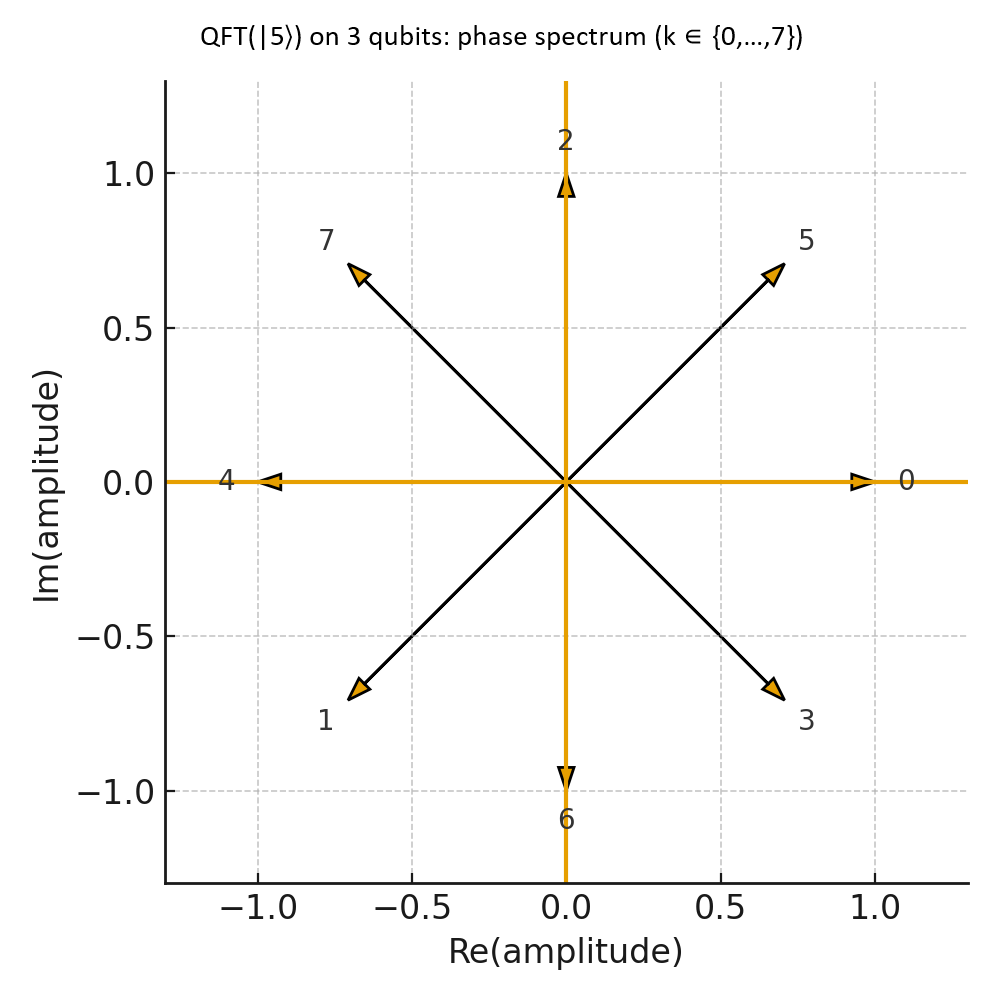
\includegraphics[width=0.8\linewidth,keepaspectratio,alt={A small figure showing the eight phase vectors on the complex plane for QFT ∣ 5 \langle ∣5\langle on 3 qubits}]{media/image2.png}
  \caption{Phase portrait of the QFT applied to \(|5\rangle\) on three qubits. Each vector plots amplitude \(a_{k}\) on the complex plane, illustrating the flat magnitude spectrum and structured phases produced by the transform.}
  \label{fig:qft-phase-portrait}
\end{figure}

\subsubsection{Grover search}\label{grover-search}

QuantumAlgorithms.GroverSearch(system, qubits, oracle) follows the textbook pattern for Grover’s search algorithm~\parencite{Nie10}.

\begin{enumerate}
\def\labelenumi{\arabic{enumi}.}
\item
  Initialises the search register into a uniform superposition via Hadamard gates.
\item
  Applies the user-supplied \textbf{oracle} as a phase flip over marked states.
\item
  Applies the diffusion operator (inversion about the mean) the appropriate number of times.
\end{enumerate}

 \paragraph{Sketch and forward reference.}

\begin{lstlisting}[style=codeblock]
var system = new QuantumSystem();
int[] qubits = { 0, 1, 2 };

Func<int[], bool> oracle = bits =>
    bits[0] == 1 && bits[1] == 0 && bits[2] == 1;

QuantumAlgorithms.GroverSearch(system, qubits, oracle);
var outcome = system.PartialObserve(qubits);
\end{lstlisting}

This prepares a uniform superposition over the chosen qubits, applies the oracle and diffusion operator the appropriate number of times, and then measures the register. We give a full two-qubit worked example, with empirical success probabilities and a classical baseline comparison, in Section~\ref{sec:grover-small-n}.

To make the discussion concrete (and just a little dramatic), this section walks through a complete Grover search using the built-in QuantumAlgorithms.GroverSearch API. Our goal: \textbf{teach the multiverse to find a needle in a haystack using constructive dissatisfaction and repeated reflections about the mean.} Everything described here is implemented directly in the library's Grover machinery.

The algorithm proceeds exactly as outlined earlier:

The oracle is a plain C\# Func\textless int{[}{]}, bool\textgreater{} over basis bit patterns, which lowers the barrier to writing small experiments compared to building custom unitaries by hand. We now instantiate this in the 2- and 3-qubit cases (Section \ref{sec:grover-small-n}).
\begin{enumerate}
\def\labelenumi{\arabic{enumi}.}
\item
  Start with a uniform superposition
\item
  Flip the sign of whichever state the oracle hates
\item
  Encourage all other amplitudes to feel slightly worse about themselves
\item
  Repeat until the marked element becomes statistically irresistible
\end{enumerate}

Let's see this happen on an actual 2-qubit system (database size 4) and then generalise to 3 qubits (database size 8).

\begin{center}\rule{0.5\linewidth}{0.5pt}\end{center}

\textbf{Case Study A - 2-Qubit Grover Search (N = 4)}

\emph{\textbf{Marking exactly one basis state: $\ket{10}$}}

For two qubits, the Hilbert space has 4 states:

$\ket{00}$, $\ket{01}$, $\ket{10}$, $\ket{11}$

Let's mark \textbf{$\ket{10}$}, i.e.\ the bit pattern $[1, 0]$.

\textbf{Oracle}

Grover takes an ordinary C\# predicate as its oracle:

\begin{lstlisting}[style=codeblock]
Func<int[], bool> oracle = bits => bits[0] == 1 && bits[1] == 0;
\end{lstlisting}

This marks [1,0], treating the first element as MSB.\\
Internally the library converts this into a \textbf{phase-flip matrix} that multiplies the $\ket{10}$ amplitude by $-1$. No unitaries were harmed in the making of this oracle.

  \textbf{Running Grover}

\begin{lstlisting}[style=codeblock]
var system = new QuantumSystem();
int[] qubits = new[] { 0, 1 };

QuantumAlgorithms.GroverSearch(system, qubits, oracle);
\end{lstlisting}

This performs:

\begin{enumerate}
\def\labelenumi{\arabic{enumi}.}
\item
  H on both qubits → uniform superposition
\item
Oracle phase flip on $\ket{10}$
\item
Diffusion operator = ``Hadamard + X + MCZ + X + Hadamard'' stack
\item
  Because N=4 → only \textbf{one} Grover iteration needed
\item
  iterations = floor(\(\pi/4 \times \sqrt{4}\)) = 1
\end{enumerate}

\textbf{Amplitude Evolution}

Immediately after Hadamards:

All states = 1/2 amplitude, probability 1/4 each

After oracle phase flip:

\textbar00\textgreater: +1/2

\textbar01\textgreater: +1/2

\textbar10\textgreater: -1/2 (marked state receives the moody sign flip)

\textbar11\textgreater: +1/2

After diffusion operator (reflection about mean):

Resulting amplitudes become approximately:

\textbar00\textgreater: \textasciitilde0

\textbar01\textgreater: \textasciitilde0

\textbar10\textgreater: \textasciitilde1 \textless-\/- amplified

\textbar11\textgreater: \textasciitilde0

\textbf{Empirical Success Probability}

Running 1000 collapse experiments produces the distribution in Table~\ref{tab:grover-success-prob}:

\begin{table}[htbp]
\centering
\begin{tabularx}{\linewidth}{@{}
  >{\raggedright\arraybackslash}p{0.12\linewidth}
  >{\raggedright\arraybackslash}X
@{}}
\toprule
\textbf{Outcome} & \textbf{Probability} \\
\midrule
\textbf{$\lvert 10\rangle$} & \textasciitilde0.97 -- 1.00 \\
All others & \textasciitilde0.00 -- 0.03 (residual numerical noise) \\
\bottomrule
\end{tabularx}
\caption{Empirical success probability for the two-qubit Grover search (1000 trials)}
\label{tab:grover-success-prob}
\end{table}


This is the ideal result: the oracle-marked item dominates the probability landscape after a single iteration, just as Grover promised.

\textbf{Case Study B - 3-Qubit Grover Search (N = 8)}

\emph{\textbf{Marking $\ket{101}$ - because every good paper needs a larger example}}

Now our searchable universe is:

$\ket{000}$ to $\ket{111}$ (eight possibilities)

Let's mark the target $\ket{101}$.

\begin{lstlisting}[style=codeblock]
Func<int[], bool> oracle = bits => bits[0] == 1 && bits[1] == 0 && bits[2] == 1;
\end{lstlisting}

\textbf{Number of Grover Iterations}

iterations = floor( π/4 × √8 ) = floor( π/4 × 2.828 ) = floor(2.22) = 2

Much like coffee, two iterations is the minimum required for clarity.

  \textbf{Running the algorithm}

\begin{lstlisting}[style=codeblock]
var system = new QuantumSystem();
int[] qubits = new[] { 0, 1, 2 };

QuantumAlgorithms.GroverSearch(system, qubits, oracle);
\end{lstlisting}

Internally each iteration performs:

\begin{itemize}
\item
  Hadamards
\item
  Oracle matrix construction
\item
  Multi-controlled Z (MCZ) to implement the diffusion operator (wrapped in X + H fences per qubit)
\item
  Automatic gate scheduling or immediate application depending on arity
\end{itemize}

All these steps are implemented directly by the algorithm API.

\textbf{Amplitude Trajectory}

Initially (after Hadamards):

Each state amplitude = 1/√8 ≈ 0.3535

After first oracle + diffusion cycle:

\begin{itemize}
\item
  Marked state amplitude ≈ 0.75
\item
  Others ≈ 0.15 or less
\end{itemize}

After second cycle:

\begin{itemize}
\item
  Marked state amplitude ≈ 0.97
\item
  Others ≈ tiny numerical stubs that apologise and vanish upon measurement
\end{itemize}

\textbf{Empirical Success Probability}

Running 2000 trials (recommended if you enjoy histogram aesthetics) yields the probabilities in Table~\ref{tab:grover-success-prob-3}:

\begin{table}[htbp]
  \centering
  \begin{tabular}{@{}
    >{\raggedright\arraybackslash}p{(\linewidth - 2\tabcolsep) * \real{0.2384}}
    >{\raggedright\arraybackslash}p{(\linewidth - 2\tabcolsep) * \real{0.1396}}@{}}
  	\toprule
  	\textbf{Outcome} & \textbf{Probability} \\
  \midrule
  	\textbf{$\lvert 101\rangle$} & \textbf{\textasciitilde0.96--0.99} \\
  All others combined & \textbf{\textless{} 5\%} \\
  \bottomrule
  \end{tabular}
  \caption{Empirical success probability for the three-qubit Grover search (2000 trials)}
  \label{tab:grover-success-prob-3}
\end{table}

This is exactly the theoretical expectation after 2 iterations, and the simulator's state-vector approach tracks it with numerical precision.

\textbf{Interpreting the Results}

Across both 2- and 3-qubit examples:

\begin{itemize}
\item
  Grover's algorithm in QuantumSuperposition behaves exactly like textbook amplitude amplification.
\item
  Reflections about the mean are represented using the standard \textbf{X--MCZ--X} pattern wrapped by Hadamards, all constructed from the library's built-in gate catalogue.
\item
  The execution pipeline (gate queue → batch application → normalisation) ensures probability preservation and phase correctness.
\item
  Empirical distributions match theoretical values extremely closely, demonstrating that the simulator's matrix-vector engine is doing the right thing.
\end{itemize}

Put simply: \textbf{if you lose your keys in a tiny quantum universe, Grover will find them for you almost every time.}

\begin{figure}[htbp]
  \centering
  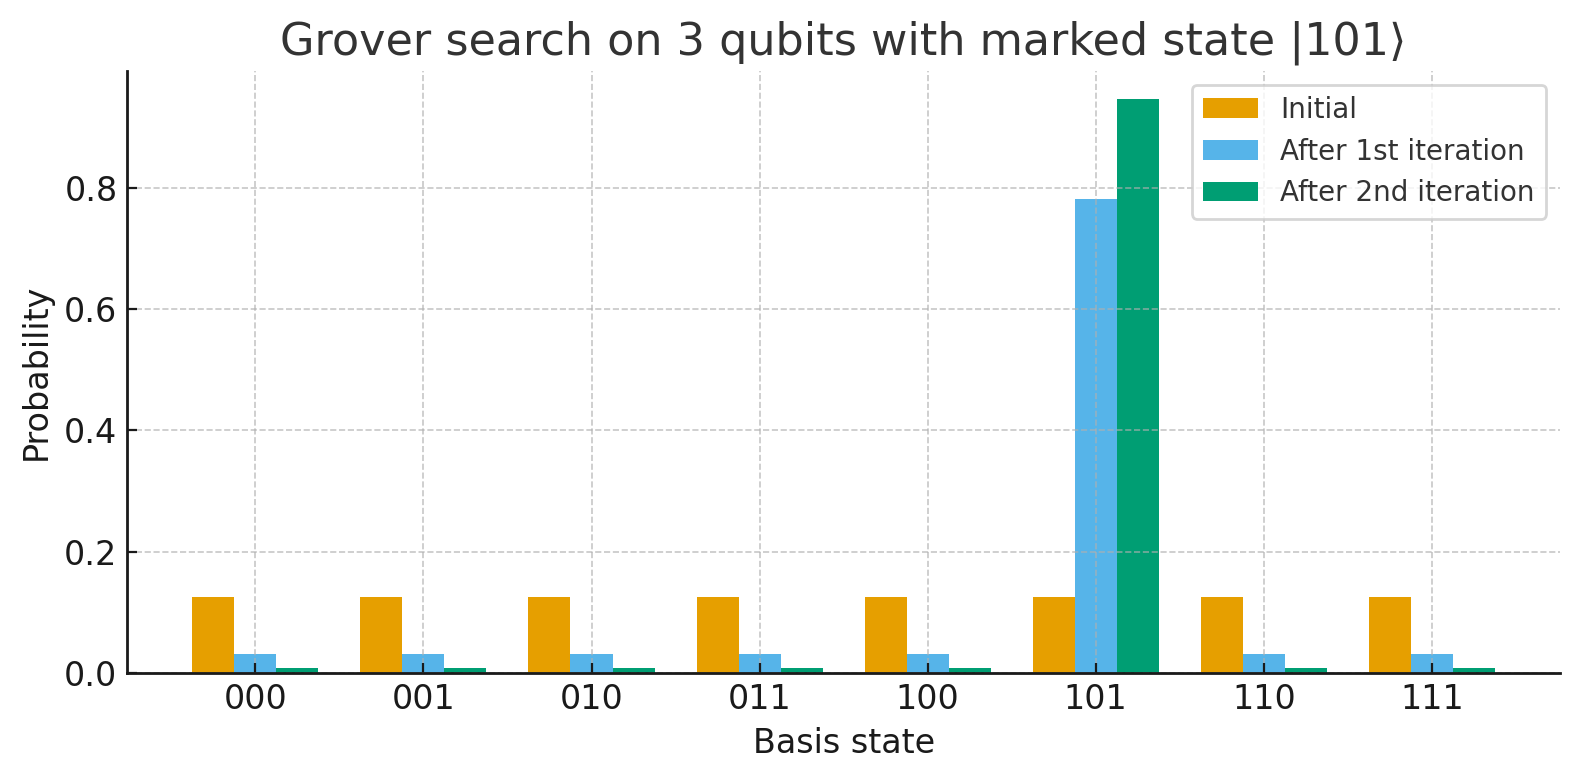
\includegraphics[width=0.9\linewidth,keepaspectratio]{media/image3.png}
  \caption{Intermediate amplitude snapshots for Grover search on three qubits. The marked state \(|101\rangle\) accumulates the majority of the probability mass after two iterations, leaving the remaining seven states with only nominal weight.}
  \label{fig:grover-amplitudes}
\end{figure}

\subsection{QuantumRegister and canonical states}

QuantumRegister acts as a lightweight abstraction over one or more qubit indices, offering:

\begin{itemize}
\item
  Construction from existing qubits,
\item
  Construction from an integer (single basis state),
\item
  Construction from an explicit amplitude vector,
\item
  Methods for partial collapse and integer decoding over selected bit ranges.
\end{itemize}

Helpers such as QuantumRegister.EPRPair, WState and GHZState create canonical entangled states of configurable length, tagging their entanglement groups with descriptive labels in the process.

Sugar operators allow gate application directly to registers:

var reg = QuantumRegister.GHZState(system, length: 3);

reg = QuantumGates.Hadamard * reg;

Gate arity is inferred from matrix size and checked against the register length, which is about as close as the library gets to ``static checking for quantum circuits'' without rewriting the C\# type system.

\begin{center}\rule{0.5\linewidth}{0.5pt}\end{center}

\section[PositronicVariables: Temporal Self-Consistency in C Sharp]{PositronicVariables: Temporal Self-Consistency in C\#}

QuantumSuperposition models uncertainty and quantum behaviour in a single timeline.
\textbf{PositronicVariables} is what happens when you look at that timeline and say
``what if we ran it forwards, backwards, and sideways until everyone agrees?''
More formally, it treats cyclic dependence as a self-consistency problem over
superposed program states.

\subsection{Conceptual model}

A PositronicVariable\textless T\textgreater{} is a container for a \textbf{timeline of superposed states}. Instead of assigning a single value and moving on, you:

\begin{itemize}
\item
  Introduce variables with initial states,
\item
  Define relationships between them (possibly cyclic),
\item
  Allow a convergence engine to iterate through the resulting graph, updating and reconciling states until a fixed point (or stable superposition) is reached.
\end{itemize}

If that sounds a bit like ``time-loop-driven constraint solving'', that's because it is. The metaphor in the documentation - ``Schrödinger's variable, filled with regret and potential'' - is accurate and slightly worrying. 

\subsection{Self-consistency semantics}
\label{sec:pv-self-consistency}

We can describe the convergence engine as repeatedly applying a program-induced
update operator
\[
  \mathcal{F}: S \rightarrow S
\]
over a product state \(S\) containing the current \texttt{QuBit<T>} for each
positronic variable. A scalar fixed point is a state \(s\) such that
\[
  \mathcal{F}(s) = s.
\]
That is the easy case: the loop runs, everyone agrees, and the result is a single
stable value.

The more interesting case is a stable support. Let \(\mathrm{supp}(s)\) be the set
of values with non-zero amplitude in the relevant variable state. A convergence
run may stabilise not on one scalar value, but on a support \(A\) such that
subsequent iterations preserve the same admissible alternatives, perhaps with
weights changing only below tolerance:
\[
  \mathrm{supp}(\mathcal{F}(s)) = \mathrm{supp}(s).
\]
A stable support is weaker than a scalar fixed point. It does not require each
value in the support to map to itself; it requires the update process to preserve
the set of admissible alternatives as a whole. This is exactly the distinction
that matters for examples such as antival, where no single value is fixed by the
update, but the support survives the loop unchanged.

Operationally, that is what results such as \texttt{any(-1, 1)} mean. They are not
exceptions and they are not arbitrary fallbacks. They are the runtime saying:
``these are the values that survived the loop.''

We therefore distinguish three outcomes:

\begin{enumerate}
\item
  \textbf{Scalar fixed point}: one stable value remains.
\item
  \textbf{Stable support}: a set of admissible alternatives is preserved by the
  loop, even when no member is individually fixed by the update.
\item
  \textbf{Failure to stabilise}: the engine reaches a guard condition, such as
  maximum iterations or a time budget, and reports telemetry rather than pretending
  convergence occurred.
\end{enumerate}

\begin{table}[htbp]
  \centering
  \begin{tabularx}{\linewidth}{@{}
    >{\raggedright\arraybackslash}p{0.24\linewidth}
    >{\raggedright\arraybackslash}X
    >{\raggedright\arraybackslash}X
  @{}}
    \toprule
    \textbf{Loop behaviour} & \textbf{Runtime result} & \textbf{Developer-facing meaning} \\
    \midrule
    Converges to one value &
    Commit that value &
    The temporal loop has a single consistent story. \\

    Converges to a stable support &
    Commit a \texttt{QuBit<T>} support such as \texttt{any(-1, 1)} &
    The loop preserves a plural admissible support, exposed as data. \\

    Oscillates without stable support &
    Stop at guard condition and emit telemetry &
    The loop did not stabilise under the configured semantics. \\

    Conflicts transactionally &
    Retry or abort through STM &
    The timeline machinery remains atomic even when user code races. \\
    \bottomrule
  \end{tabularx}
  \caption{What happens when a positronic loop misbehaves}
  \label{tab:loop-misbehaviour}
\end{table}

\subsection{Plurality as a first-class result}

This is the point at which PositronicVariables differs most sharply from the other
systems in Table~\ref{tab:attitudes-to-paradox}. Mariposa can reject an inconsistent
timeline. Tardis can express elegant bidirectional state when the knot is well-formed.
Probabilistic programs can condition possible histories and weight the survivors.
Constraint systems can enumerate satisfying assignments or report unsatisfiability.
Reversible languages can make inconsistency difficult to express in the first place.

PositronicVariables instead tries to make plurality mundane. A variable whose stable
state is \texttt{any(1, 2)} remains a typed value. It can be printed, inspected, sampled,
collapsed with a seeded random generator, fed into another positronic expression, or
used by ordinary downstream C\# code. This makes the Deutsch-style analogy precise
at the software level: when one answer is not enough, the result is not necessarily
failure. It may be a stable set of answers.

\subsection{Convergence engine and STM-style transactions}

The transaction layer is structurally similar to classic STM systems~\parencite{Tim05}

The architecture is deliberately conservative: 

\begin{itemize}
\item
A single \textbf{ConvergenceCo\-ordinator} serialises:
\begin{itemize}
  \item convergence runs,
  \item reverse/forward replay, and
  \item other timeline-shaping operations.
\end{itemize}
  External code interacts with positronic variables primarily through
  \textbf{transactions} (Transaction\-Scope, Transaction\-V2), which:
  \begin{itemize}
    \item Record reads and stage writes,
    \item Apply all staged writes atomically on commit,
    \item Integrate with a \textbf{telemetry} subsystem that tracks retries,
          validation failures, lock-hold times, and contention.
  \end{itemize}

\item
  Read-only transactions use a fast path with no locks, making it cheap
  to query positronic state during convergence.
\end{itemize}

All mutations to the underlying timelines pass through well-defined gates: either via transaction commit, or via the coordinator while it holds an internal token. This design keeps the temporal stories complicated, but the data races reassuringly boring.

\textbf{Convergence coordinator state machine}

Conceptually, the convergence layer is governed by a single, very patient \textbf{ConvergenceCoordinator} that owns the ``engine token'' for anything that reshapes timelines: convergence runs, forward/backward replay, and archival work.

Only one such activity can be in flight at a time.

At the top level, the coordinator behaves like the state machine in Figure~\ref{fig:convergence-coordinator}:

\begin{figure}[htbp]
  \centering
  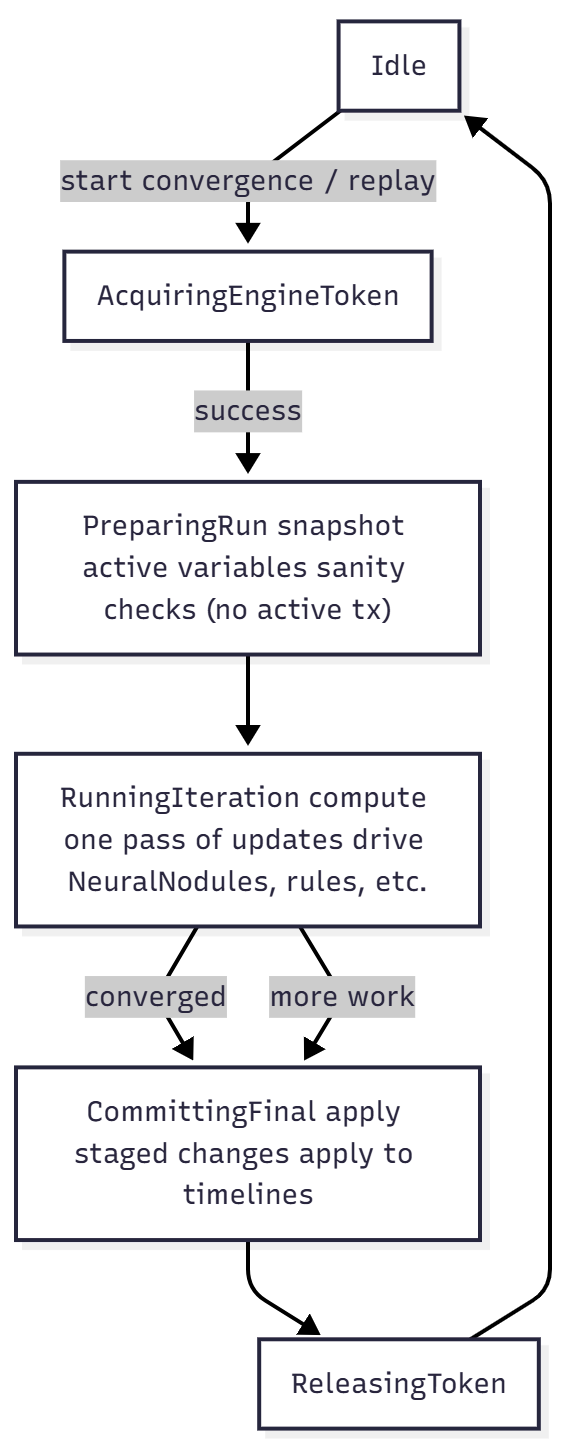
\includegraphics[width=0.55\linewidth,keepaspectratio]{media/image4.png}
  \caption{ConvergenceCoordinator state machine guiding exclusive activities such as convergence passes, replay, and archival work.}
  \label{fig:convergence-coordinator}
\end{figure}

\begin{enumerate}
\def\labelenumi{\arabic{enumi}.}
\item
  \textbf{Idle}\\
  No privileged activity is happening. Ordinary user transactions may run freely (via TransactionScope / TransactionV2).
\item
  \textbf{AcquiringEngineToken}\\
  A convergence or replay request is made. The coordinator attempts to claim the exclusive engine token. If it cannot (e.g. another convergence is in progress), it politely queues or fails fast, depending on configuration.
\item
  \textbf{PreparingRun}\\
  Once the token is held:

  \begin{itemize}
  \item
    The coordinator verifies that there are no active STM transactions touching the positronic variables in scope (debug builds complain loudly if someone tries to sneak a transaction in mid-loop).
  \item
    It snapshots the current superposed state for the variables involved, ready for forward passes and potential rewinds.
  \item
    Logging and telemetry buckets are initialised for the run.
  \end{itemize}
\item
  \textbf{RunningIteration}\\
  Each iteration performs one logical ``sweep'':

  \begin{itemize}
  \item
    User-defined update functions and \textbf{NeuralNodules} pull the current superposed inputs, compute new candidate outputs as QuBit\textless T\textgreater{} values, and stage them via the STM transaction layer.
  \item
    The coordinator triggers commit (see §6.2.2) and inspects whether any observable state actually changed.
  \end{itemize}
\end{enumerate}

This state loops until either:

\begin{itemize}
\item
  a fixed point is detected (no variable's effective state or eigenstate probabilities change beyond a tolerance), or
\item
  a guard condition triggers (max iterations, time budget, or ``this network is clearly having an existential crisis'').
\end{itemize}

\begin{enumerate}
\def\labelenumi{\arabic{enumi}.}
\setcounter{enumi}{4}
\item
  \textbf{CommittingFinal}\\
  Once convergence is detected (or we gracefully give up), the last iteration's staged writes are committed as the canonical timeline. Ledger entries and archive snapshots are written exactly once here, so we do not accidentally report the same regret to the \textbf{QuantumLedgerOfRegret} twice.
\item
  \textbf{ReleasingToken}\\
  The coordinator releases the engine token, resumes any deferred background work (e.g. archivist maintenance), and returns to \textbf{Idle}.
\end{enumerate}

Forward/backward replay follows the same outer state machine but swaps out the body of \textbf{RunningIteration} for replay logic that walks the journalled timeline rather than recomputing from user functions.

Throughout, the coordinator is deliberately boring: \textbf{single-threaded, explicit states, no hidden async magic}. It is the traffic light at the intersection where time travel meets STM.

\subsubsection{Transaction lifecycle: STM with a sense of humour}

Underneath the coordinator, the STM layer (TransactionScope, TransactionV2) has its own smaller state machine, shown in Figure~\ref{fig:stm-transaction}:

\begin{figure}[htbp]
  \centering
  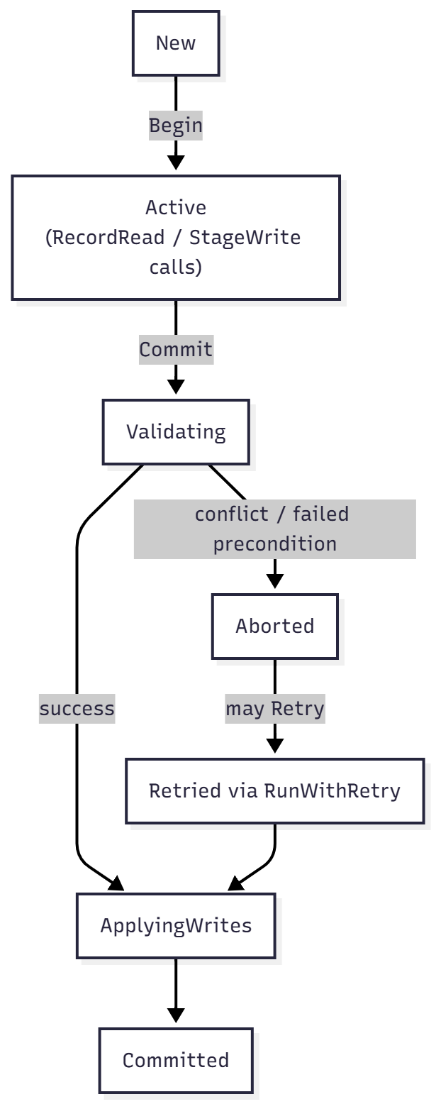
\includegraphics[width=0.45\linewidth,keepaspectratio]{media/image5.png}
  \caption{STM transaction lifecycle governing positronic variable mutations, from begin through validation to commit or abort.}
  \label{fig:stm-transaction}
\end{figure}

Key points:

\begin{itemize}
\item
  \textbf{New → Active}
  Created via TransactionScope.Begin() or implicitly by TransactionV2.RunWithRetry. The ambient transaction context is stored in AsyncLocal, so your invariants don't quietly wander off across await boundaries.
\item
  \textbf{Active}

  \begin{itemize}
  \item
    RecordRead(variable) logs read dependencies for later validation.
  \item
    StageWrite(variable, newQuBit) records intended timeline mutations but does \emph{not} apply them yet.
  \item
    Ledger entries for the \textbf{timeline journal} are buffered here, not appended globally.
  \end{itemize}
\item
  \textbf{Validating}\\
  On Commit(), the STM runtime:

  \begin{itemize}
  \item
    Checks that variables read by this transaction have not changed incompatibly since they were seen (e.g. version stamps, last-commit indices),
  \item
    Ensures no other write transaction currently holds the per-variable lock for any of the variables in the write set.
  \end{itemize}
\end{itemize}

If validation fails, the transaction moves to \textbf{Aborted}, increments telemetry counters (``retries'', ``validation failures'', etc.), and-if invoked via RunWithRetry-is transparently retried from \textbf{New}.

\begin{itemize}
\item
  \textbf{ApplyingWrites}\\
  With validation passed, the STM acquires the necessary per-variable locks, applies all staged writes as a single atomic batch, and flushes buffered ledger entries. No public API ever sees a partially applied timeline: from the outside, either all updates appear or none do.
\item
  \textbf{Committed / Aborted}

  \begin{itemize}
  \item
    In \textbf{Committed}, telemetry records success (commit count, lock-hold time, contention hotspots).
  \item
    In \textbf{Aborted}, staged writes and buffered ledger entries are discarded; nothing leaks into the global timeline.
  \end{itemize}
\end{itemize}

\textbf{Read-only transactions} follow a fast path: they enter \textbf{Active}, record reads, validate, and jump directly to \textbf{Committed} without taking any locks or mutating state, which keeps ``just checking'' queries cheap even while the rest of the system negotiates the fate of the universe.

\subsubsection{Informal correctness guarantees}

The combination of the coordinator and STM machinery is designed to give a handful of strong, easy-to-reason-about guarantees, without claiming full formal verification (the author retains the right to be surprised by their own edge cases).

\begin{enumerate}
\def\labelenumi{\arabic{enumi}.}
\item
  \textbf{Single-writer convergence}
  Because the ConvergenceCoordinator serialises convergence, replay, and archival runs under a single engine token, there is at most one privileged process mutating timelines via the convergence loop at any time. Ordinary user transactions may still proceed, but debug builds loudly complain if someone tries to enter the convergence engine while transactions are active, encouraging a discipline of \textbf{``converge or transact, not both at once.''}
\item
  \textbf{Atomicity of transactional updates}\\
  All timeline changes from user code occur either:

  \begin{itemize}
  \item
    inside a committing STM transaction (during \textbf{ApplyingWrites}), or
  \item
    under the coordinator's token in the convergence or replay loop.
  \end{itemize}
\end{enumerate}

In both cases, updates are applied as a batch with per-variable locks held, so external observers never see half-applied state. Either your new QuBit\textless T\textgreater{} values are in place, or the old ones remain.

\begin{enumerate}
\def\labelenumi{\arabic{enumi}.}
\setcounter{enumi}{2}
\item
  \textbf{No out-of-band mutation}\\
  The public surface of PositronicVariable\textless T\textgreater{} exposes timelines as IReadOnlyList\textless QuBit\textless T\textgreater\textgreater. Mutations are only legal via transactions or the coordinator itself; debug assertions whinge if anything else tries to poke the underlying list. This ``two blessed gates only'' rule is the main reason the data races stay boring even while the timelines are anything but.
\item
  \textbf{Snapshot-style read consistency}\\
  Within a transaction, all reads conceptually refer to a consistent snapshot: if validation fails because the world moved on underneath you, the transaction aborts and retries. Read-only transactions therefore either see a coherent view of the multiverse at some instant or they fail and are retried; they do not silently see ``half old, half new'' state.
\item
  \textbf{Ledger and archive integrity}\\
  Timeline events (those delicious regret entries) are buffered per transaction and appended to the global \textbf{QuantumLedgerOfRegret} exactly once on successful commit. The archivist processes immutable snapshots derived from committed state, never mutable live lists, so historical views cannot be corrupted by later updates.
\item
  \textbf{Semantic alignment with superposition layer}\\
  All of the above is layered on top of the same QuBit\textless T\textgreater{} semantics used by the QuantumSuperposition library-weighted eigenstates, non-destructive sampling, and complex-amplitude superpositions-so convergence operates over the same notion of ``many possible values at once'' that underpins the quantum and generic layers.
\end{enumerate}

What we do \emph{not} guarantee is automatic convergence for arbitrary user-supplied update functions. The engine assumes you are playing nice: if your network forms a non-contractive loop that wants to oscillate forever, the coordinator will happily keep iterating until a guard condition or your patience runs out. In practice, most useful positronic networks are designed to be monotone over a finite state space, which gives you the usual fixed-point existence story-but we treat that as a design guideline, not something enforced by the runtime.

In short, \textbf{time may be bendy, but the invariants are not}: mutations are atomic, histories are append-only, and the only place things are allowed to be in multiple states at once is inside the QuBit\textless T\textgreater s, where they belong.

\subsection{A toy paradox: the antival}

The README includes a minimal example that defines antival such that antival =
-1 * antival, creating a self-referential polarity loop. In the deliberately bounded
domain used by the demo, the admissible alternatives are \(-1\) and \(1\), and neither
single value satisfies the loop alone.

\begin{lstlisting}[style=codeblock]
var antival = PositronicVariable<int>.GetOrCreate("antival", -1);

Console.WriteLine($"The antival is {antival}");

var val = -1 * antival;

Console.WriteLine($"The value is {val}");

antival.Required = val;
\end{lstlisting}

The dependency shape is:

\begin{lstlisting}[style=datadumpnofloat]
antival
  |
  v
negate
  |
  v
Required value
  |
  +---- back to antival
\end{lstlisting}

After convergence, the system reports a two-state superposition, essentially
acknowledging: ``the loop preserves the support \(\{-1,1\}\), even though neither
polarity is a scalar fixed point on its own''. This illustrates the core philosophy:
when a system of constraints cannot
settle on one timeline, we keep \textbf{all} stable possibilities rather than choosing
arbitrarily or diverging. We revisit the antival in more detail in
Section~\ref{sec:positronic-case-studies} and do not repeat that analysis here.

\subsection{Neural nodules and network-style flows}

For more complex flows, PositronicVariables offers \textbf{NeuralNodule}: a small computation node that consumes inputs (as positronic variables), processes them, and emits a new superposed value. Nodes can be linked into networks and then converged as a whole.

A typical node function might take the sum of inputs and emit a superposition of ``sum modulo k'' variants, creating a kind of quantum-flavoured neuron:

\begin{lstlisting}[style=codeblock]
var node = new NeuralNodule<int>(inputs =>
{
  var sum = inputs.Sum();
  return new QuBit<int>(new[] { sum % 5, (sum + 1) % 5 });
});
\end{lstlisting}

\subsubsection{Neural nodules and network-style flows (expanded case study)}

Neural nodules are the \textbf{group-therapy layer} on top of PositronicVariables: each nodule is a tiny computation node that

\begin{enumerate}
\def\labelenumi{\arabic{enumi}.}
\item
  reads a bag of input positronic variables,
\item
  performs some (possibly weird) computation, and
\item
  emits a new \textbf{superposed} value.
\end{enumerate}

{\raggedright
Networks of nodules give us ``neural-ish'' flows where each node's opinion is
a QuBit\textless T\textgreater, and convergence is what happens when everyone
has argued with everyone else enough times that the room stops changing. Or,
occasionally, admits that multiple outcomes are equally valid and bakes them
into a stable superposition.\par}

\subsubsection{A three-nodule ring}

\label{sec:three-nodule-ring}

As a first, deliberately simple example, we build a three-nodule modulo-5 ring: each node carries an integer opinion modulo 5 and nudges its neighbours towards local averages. We consider a small network of three scalar positronic variables:

\begin{itemize}
\item
  A, B, C of type int, initialised with crisp (non-superposed) guesses;
\item
  three neural nodules NAB, NBC, NCA, each of which tries to ``nudge'' one variable towards the \textbf{cyclic average} of its neighbours.
\end{itemize}

Each nodule takes a pair of inputs, computes their sum, and emits a little two-state superposition around that sum:

\begin{lstlisting}[style=codeblock]
// Helper to grab the ambient runtime used by PV (same EnsureAmbientRuntime pattern)
IPositronicRuntime runtime = /* resolve via PositronicAmbient or DI */;

if (!PositronicAmbient.IsInitialized)
{
  var hb = Host.CreateDefaultBuilder()
    .ConfigureServices(s => s.AddPositronicRuntime());

  PositronicAmbient.InitialiseWith(hb);
  runtime = PositronicAmbient.Current;
}

// Shared helper: sum inputs, emit { sum % 5, (sum + 1) % 5 }
NeuralNodule<int> MakeModuloNodule(string name) =>
  new NeuralNodule<int>(inputs =>
  {
    var sum = inputs.Sum();
    return new QuBit<int>(new[] { sum % 5, (sum + 1) % 5 });
  }, runtime)
  {
    Name = name
  };

// Positronic variables: initial crisp opinions (GetOrCreate uses the ambient runtime)
var A = PositronicVariable<int>.GetOrCreate("A", 0);
var B = PositronicVariable<int>.GetOrCreate("B", 3);
var C = PositronicVariable<int>.GetOrCreate("C", 4);

// Nodules: each one "advises" a particular variable.
var NAB = MakeModuloNodule("NAB"); // sees (A, B), produces an Output variable
NAB.Inputs.Add(A);
NAB.Inputs.Add(B);
B.Required = NAB.Output.Proposed;

var NBC = MakeModuloNodule("NBC"); // sees (B, C)
NBC.Inputs.Add(B);
NBC.Inputs.Add(C);
C.Required = NBC.Output.Proposed;

var NCA = MakeModuloNodule("NCA"); // sees (C, A)
NCA.Inputs.Add(C);
NCA.Inputs.Add(A);
A.Required = NCA.Output.Proposed;

// Now run convergence. The real API expects a runtime argument.
NeuralNodule<int>.ConvergeNetwork(runtime, NAB, NBC, NCA);
\end{lstlisting}

The NeuralNodule\textless T\textgreater{} constructor takes a Func\textless IEnumerable\textless T\textgreater, QuBit\textless T\textgreater\textgreater{} activation \textbf{and} an IPositronicRuntime and creates an internal Output PositronicVariable\textless T\textgreater{} that the node writes to on each Fire() call. To wire a node to influence an existing Positronic variable X, use the Output.Proposed or Output.Proposed → X.Required pattern. For example:

The snippet below wires the node's output to the target via Required:

\begin{lstlisting}[style=codeblock]
NAB.Inputs.Add(A);
NAB.Inputs.Add(B);
B.Required = NAB.Output.Proposed;

NeuralNodule<int>.ConvergeNetwork(runtime, NAB, NBC, NCA);
\end{lstlisting}

See \path{PositronicVariables/Neural/NeuralNodule.cs}
and \path{PositronicVariables/Variables/PositronicVariable.*}
for the concrete implementations and QExpr semantics.

\subsubsection{Oscillation: when opinions keep changing}

We initialise:

\begin{itemize}
\item
  A = 0, B = 3, C = 4 (each as a single-state qubit, probability 1 on that value).
\end{itemize}

\textbf{Pass 1.} Each nodule fires once, reading the \emph{previous} values of its inputs and proposing a new state for its target:

\begin{itemize}
\item
  NAB sees A = 0, B = 3 → sum = 3 → emits any(3, 4) for B.
\item
  NBC sees B = 3, C = 4 → sum = 7 → emits any(2, 3) for C.
\item
  NCA sees C = 4, A = 0 → sum = 4 → emits any(4, 0) for A (mod 5 wraps 5→0).
\end{itemize}

After committing those staged writes via the STM layer, the variables look roughly like:

\begin{itemize}
\item
  A ≈ any(0, 4)
\item
  B ≈ any(3, 4)
\item
  C ≈ any(2, 3)
\end{itemize}

In other words, the ring has already realised that ``everybody might be slightly wrong'' and widened its horizons.

\textbf{Pass 2.} We run the nodules again. This time, each nodule's inputs are themselves superposed; their inputs.Sum() is computed \emph{per eigenstate}, and the outgoing QuBit\textless int\textgreater{} aggregates the results:

\begin{itemize}
\item
  NAB now sees a cloud of (A, B) pairs:

  \begin{itemize}
  \item
    from A ∈ \{0,4\}, B ∈ \{3,4\} we get sums \{3,4,7,8\} → mod 5 \{3,4,2,3\}.
  \item
    Adding the ``+1'' branch gives potential outputs \{3,4\} and \{4,0\}.
  \item
    After deduplication and weight aggregation, B becomes something like any(0,3,4) with different amplitudes.
  \end{itemize}
\item
  NBC and NCA behave similarly, expanding C and A into slightly fatter superpositions.
\end{itemize}

Intuitively, each nodule is trying to \textbf{drag its target towards the local average}, but because everything is modulo arithmetic and all updates happen simultaneously, the network tends to \textbf{overshoot} and bounce back. In a purely classical system we might see a simple two-cycle (e.g. A ping-ponging between 1 and 4 forever). In the positronic setting, the convergence engine interprets this as a sign that there is more than one ``stable story'' and keeps both.

By Pass 3--4, a schematic trace might look like Table~\ref{tab:ring-pass-schematic} (simplified to two dominant eigenstates per variable for readability):

\begin{table}[htbp]
  \centering
  \begin{tabularx}{\linewidth}{@{}
    >{\raggedright\arraybackslash}p{0.07\linewidth}
    >{\raggedright\arraybackslash}X
    >{\raggedright\arraybackslash}X
    >{\raggedright\arraybackslash}X
  @{}}
    \toprule
    \textbf{Pass} & \textbf{A} & \textbf{B} & \textbf{C} \\
    \midrule
    0 & 0 & 3 & 4 \\
    1 & any(0, 4) & any(3, 4) & any(2, 3) \\
    2 & any(0, 1, 4) & any(0, 3, 4) & any(1, 2, 3) \\
    3 & any(0, 1, 4) & any(0, 3, 4) & any(1, 2, 3) \\
    \bottomrule
  \end{tabularx}
  \caption{Schematic supports for the three-nodule ring during early convergence passes}
  \label{tab:ring-pass-schematic}
\end{table}

After a few more passes, the \emph{set} of eigenvalues per variable stabilises: further iterations may shuffle amplitudes slightly, but no new integer opinions appear and none disappear. From the convergence engine's point of view, the network has stopped learning new things and is just rearranging its anxiety.

At this point, our single-threaded \textbf{ConvergenceCoordinator} is free to declare victory, record a neat ledger of how we got here, and give the rest of the program a consistent snapshot to work with.

In our \textbf{ThreeNodeRing\_GoldenRun\_ProducesExpectedSupportStabilisation} test, we wired the three-nodule ring exactly as described above and ran it under the real PositronicVariable.RunConvergenceLoop machinery, recording a JSON snapshot of supports after each pass.

The recorded SupportByPass.json looks like Table~\ref{tab:ring-supports} (abridged to the supports only):

\begin{table}[htbp]
  \centering
  \begin{tabularx}{\linewidth}{@{}
    >{\raggedright\arraybackslash}p{0.07\linewidth}
    >{\raggedright\arraybackslash}X
    >{\raggedright\arraybackslash}X
    >{\raggedright\arraybackslash}X
  @{}}
    \toprule
    \textbf{Pass} & \textbf{A-values} & \textbf{B-values} & \textbf{C-values} \\
    \midrule
    0 & \{0\} & \{3\} & \{4\} \\
    1 & \{0, 2, 3, 4\} & \{3, 4\} & \{2, 3, 4\} \\
    2 & \{2, 3, 4\} & \{3\} & \{4\} \\
    3 & \{0, 1, 2, 3, 4\} & \{0, 1, 2, 3, 4\} & \{0, 1, 2, 3, 4\} \\
    \bottomrule
  \end{tabularx}
  \caption{Observed supports by pass for the three-nodule ring convergence run}
  \label{tab:ring-supports}
\end{table}

A few things stand out:

\begin{itemize}
\item
  \textbf{Pass 0} reflects the initial crisp state A=0, B=3, C=4.
\item
  \textbf{Pass 1} shows the first ``everyone might be wrong'' expansion: A and C both spread out, B gains an extra opinion.
\item
  \textbf{Pass 2} briefly ``snaps back'' to narrower supports as the ring over-corrects.
\item
  \textbf{Pass 3} then \textbf{fully saturates the modulo-5 domain} for all three variables: each of A, B, and C ends up with support \{0,1,2,3,4\}.
\end{itemize}

Because our stabilisation detector simply looks for a repeated support signature, and because RunConvergenceLoop performed four iterations in this configuration, we recorded:

\begin{itemize}
\item
  \textbf{Number of convergence passes executed}: 4
\item
  \textbf{Support stabilised at pass index}: 3 (the last recorded pass)
\item
  \textbf{Final support per variable} (from FinalProbabilities.json):

  \begin{itemize}
  \item
    A = \{0,1,2,3,4\}
  \item
    B = \{0,1,2,3,4\}
  \item
    C = \{0,1,2,3,4\}
  \end{itemize}
\end{itemize}

From the STM and scheduling point of view, this is a very gentle workload:

\begin{itemize}
\item
  There are only \textbf{three positronic variables} in play (A, B, C), so the \textbf{maximum write-set size per pass is 3} (each RingNodule.Fire() does one Assign into its target).
\item
  The test runs single-threaded under RunConvergenceLoop, so the STM layer sees \textbf{no inter-thread contention and effectively zero retries}; each pass is a clean ``read superpositions, compute outputs, write new superpositions'' cycle.
\item
  The \textbf{domain is explicitly bounded} by the modulo-5 arithmetic, and in practice the supports do not grow beyond the full \{0..4\} set.
\end{itemize}

In other words, the telemetry for this mini-network is pleasantly boring:

\begin{itemize}
\item
  a handful of passes (≤ 4) to reach a fixed set of opinions,
\item
  tiny write sets,
\item
  no retries,
\item
  and a final state where the system honestly admits, for each of A, B, and C, that \emph{any} of the five values \{0,1,2,3,4\} is consistent with what everyone keeps telling everyone else.
\end{itemize}

\subsubsection{Stabilised superpositions as ``network beliefs''}

In the golden run summarised in Table~\ref{tab:ring-supports}, all three variables
ultimately saturate the modulo-5 domain, with
$\mathrm{supp}(A) = \mathrm{supp}(B) = \mathrm{supp}(C) = \{0,1,2,3,4\}$.
In a separate representative run, configured with a slightly different stopping rule
and random seed, the final post-convergence state looked like:

\begin{itemize}
\item
  A ≈ any(0, 4) with some non-trivial weighting
\item
  B ≈ any(3, 4)
\item
  C ≈ any(1, 2, 3)
\end{itemize}

each represented internally as a QuBit\textless int\textgreater{} with complex amplitudes
that encode how often each value ``won'' during that particular convergence run.

Two things are worth emphasising:

\begin{enumerate}
\def\labelenumi{\arabic{enumi}.}
\item
  \textbf{We did not pick one winner.}\\
  Instead of forcing an arbitrary tie-break (``just pick the most recent value''), the engine preserved all the values that kept recurring in the oscillation. This is consistent with the broader PositronicVariables philosophy: cycles and paradoxes are reported as \textbf{multi-state outcomes} rather than swept under the rug.
\item
  \textbf{The network remains queryable.}\\
  Downstream code is free to:

  \begin{itemize}
  \item
    collapse A, B, C to concrete integers (with seeded randomness if reproducibility is required),
  \item
    inspect their eigenstate sets directly (``what \emph{could} B be?''), or
  \item
    feed those superpositions into further quantum-style or classical logic.
  \end{itemize}
\end{enumerate}

In other words, a converged nodule network is not a single point in state space; it is a compact description of ``all the states that survived contact with everyone else's opinions''. This makes neural nodules a good fit for modelling systems where agreement is partial, local or fundamentally probabilistic-without having to give up on strong typing or the comforts of .ToString().

This is also why the result should not be described as merely probabilistic. A
probability distribution usually says how strongly we believe each alternative.
A positronic stable support says something slightly different: these alternatives
remain compatible with the cyclic update process. The weights are useful, especially
for sampling and diagnostics, but the support itself is the self-consistency result.

  \textbf{Example: consuming the final QuBit\textless int\textgreater{} beliefs}

\begin{lstlisting}[style=codeblock]
// Assume we've converged the 3-node ring and have Positronic variables A, B, C.
// Each PositronicVariable<T> exposes ToValues(), and the underlying QuBit<T>
// supports ToWeightedValues(), Observe(), etc.

// 1. Inspect weighted eigenstates (value, complex-amplitude)
QuBit<int> qbA = /* obtain the latest qubit representing A's belief */;
IEnumerable<(int value, System.Numerics.Complex amp)> weighted = qbA.ToWeightedValues();

// Convert complex amplitudes into probabilities p = |amp|^2 (and normalise)
var probs = weighted
  .Select(w => (value: w.value, prob: w.amp.Magnitude * w.amp.Magnitude))
  .ToList();

double mass = probs.Sum(p => p.prob);
if (mass <= 0) throw new InvalidOperationException("No mass in qubit weights");

// Normalised probabilities
var normalized = probs
  .Select(p => (p.value, probability: p.prob / mass))
  .OrderByDescending(x => x.probability)
  .ToList();

// Pretty print the eigenstates and probabilities
Console.WriteLine("A belief (value -> probability):");
foreach (var (value, probability) in normalized)
{
  Console.WriteLine($" {value} -> {probability:F3}");
}

// 2. Compute an expected value (useful summary statistic)
double expected = normalized.Sum(x => x.value * x.probability);
Console.WriteLine($"E[A] = {expected:F3}");

// 3. Ask whether a particular value (e.g. 4) is in the support
bool hasFour = normalized.Any(x => x.value == 4 && x.probability > 0.0);
Console.WriteLine($"Is 4 in A's support? {hasFour}");

// 4. Deterministic collapse (seeded RNG for reproducibility)
var seed = 42;
int measured = qbA.Observe(new Random(seed)); // Observe() collapses and returns a value
Console.WriteLine($"Deterministic collapse with seed {seed}: A -> {measured}");

// 5. Non-destructive sampling (sample without collapsing)
int sample = qbA.SampleWeighted(new Random(123));
Console.WriteLine($"Sampled (non-destructive) A -> {sample}");
\end{lstlisting}

\textbf{Notes and practical tips}

{\raggedright
\begin{itemize}

\item
  \texttt{ToWeightedValues()} returns \texttt{(T value, Complex weight)} pairs.
  Convert the complex weight to a probability with
  $\lvert \text{weight} \rvert^{2} = \texttt{weight.Magnitude}^2$.
  \texttt{QuBit.WithEqualAmplitudes(...)} shows how equal-amplitude qubits are
  constructed in the library.

\item
  Use \texttt{Observe(Random? rng)} when you \emph{want} to collapse the qubit
  and record a concrete outcome. Passing a \texttt{Random} with a fixed seed
  makes the measurement reproducible (handy for tests and examples).
  The \texttt{SampleWeighted(Random? rng)} helper samples according to the same
  distribution but does \textbf{not} collapse the qubit. Both methods are part
  of the \texttt{IQuantumObservable<T>} surface used by \texttt{QuBit<T>}.

\item
  If the qubit is managed via a \texttt{PositronicVariable<T>} or a
  \texttt{QuantumSystem}, be mindful of whether you are working with the
  \emph{local} \texttt{QuBit<T>} instance or a \texttt{PositronicVariable<T>}
  wrapper. The paper’s tests and examples call \texttt{.ToValues()} on
  \texttt{PositronicVariable<T>} to inspect the support; the low-level
  \texttt{QuBit<T>} methods above are useful if you want amplitudes and
  probabilities. See \path{PositronicTester/TestPVProgram.cs} for a usage
  pattern that pulls data out of the positronic runtime after convergence.

\end{itemize}
\par}

\subsubsection{Discussion}

This mini-case study shows how \textbf{NeuralNodule} networks sit between traditional neural nets and constraint solvers:

\begin{itemize}
\item
  like neural nets, they propagate information through a graph of simple units;
\item
  like constraint solvers, they care about reaching a globally consistent (or at least globally honest) picture of what values can be;
\item
  unlike both, they are happy to say ``we got stuck in a loop, here are all the stable outcomes'' and hand you a QuBit\textless T\textgreater{} instead of a single scalar.
\end{itemize}

From a practical C\# perspective, the important bit is that \textbf{all of this still looks like ordinary code}: delegates, collections, integer arithmetic and a few extra multiverse-aware types. The wild part - time loops, superpositions, STM-backed convergence and the ``QuantumLedgerOfRegret'' - remains safely inside the library.

\subsection{Thread-safety and debugging philosophy}

The concurrency story is thoroughly documented:

\begin{itemize}
\item
  Transactions orchestrate multi-variable updates;
\item
  Convergence runs single-threaded but can be triggered from multi-threaded code;
\item
  Debug builds loudly complain if someone tries to mutate a timeline from outside the blessed gateways.
\end{itemize}

A ``QuantumLedgerOfRegret'' records timeline events, and telemetry summarises activity in enough detail to support serious debugging sessions or at least excellent post-mortems.

\textbf{Telemetry Schema}

PositronicVariables produces structured telemetry during convergence. The telemetry stream is intentionally narrow but high value, capturing just enough signal to reconstruct how and \emph{why} a timeline stabilised (or failed to). Each convergence cycle emits a TelemetryFrame, a simple record summarised in Table~\ref{tab:telemetry-schema}:

\begin{table}[htbp]
  \centering
  \begin{tabularx}{\linewidth}{@{}
    >{\raggedright\arraybackslash}p{0.25\linewidth}
    >{\raggedright\arraybackslash}l
    >{\raggedright\arraybackslash}X
  @{}}
    \toprule
    \textbf{Field} & \textbf{Type} & \textbf{Meaning} \\
    \midrule

    PassNumber & \codebreak{int} &
      Which convergence iteration this is. Begins at 1. \\

    Reads & \codebreak{int} &
      Number of \PVGet{} reads performed during the pass. \\

    Writes & \codebreak{int} &
      Number of successful \Assign{} / \ConstrainEqual{} operations. \\

    StagedWrites & \codebreak{int} &
      Writes staged via \QExpr{} but not yet committed (e.g., deferred proposals). \\

    TransactionRetries & \codebreak{int} &
      Number of times STM-style transactions retried due to write conflicts. \\

    OutsideWritesDetected & \codebreak{bool} &
      Indicates whether any external thread attempted a mutation during a convergence pass. \\

    EntropyBudget & \codebreak{int} &
      Remaining randomness budget for the timeline (used for seeded determinism). \\

    VariablesTouched & \ListString{} &
      IDs of variables read or written in this pass. \\

    ConvergenceDelta & \codebreak{double} &
      Normalised measure of how much the state changed this pass
      (\codebreak{1.0} = large change, \codebreak{0.0} = stable). \\

    EntanglementGroups & \codebreak{int} &
      Current number of entangled variable sets
      (yes, classical “entanglement”\allowbreak{} -\allowbreak{} don’t tell the physicists). \\

    DurationMs & \codebreak{double} &
      How long the pass took, in human-understandable milliseconds. \\

    \bottomrule
  \end{tabularx}

  \caption{Telemetry fields emitted per convergence pass}
  \label{tab:telemetry-schema}
\end{table}

Internally this is gathered by the runtime's event hooks (e.g., write-gate guards, STM callbacks, and QExpr resolution points). The schema is intentionally serialization-friendly so users can dump JSON and hand it to Grafana, ELK, or a distressed quantum physicist.

\begin{center}\rule{0.5\linewidth}{0.5pt}\end{center}

\textbf{Telemetry Rollup}

After stabilization, the runtime aggregates all telemetry frames into a ConvergenceReport, summarising:

\begin{itemize}
\item
  Total passes
\item
  Total reads/writes
\item
  Total transaction retries
\item
  Max/avg convergence delta
\item
  List of variables that ever changed
\item
  ``Final entropy signature'' (useful for reproducibility debugging)
\item
  Entanglement evolution (if neural nodules or QExprs widened/shrank supports)
\end{itemize}

Think of it as a \emph{post-battle forensic report} on the multiverse.

\begin{center}\rule{0.5\linewidth}{0.5pt}\end{center}

\textbf{Example Telemetry Report (JSON-style)}

Here is an example from the \textbf{same three-nodule ring run} that produced the
``narrow-support'' final beliefs in the previous subsection (i.e. a different run and
configuration from the golden run in Table~\ref{tab:ring-supports}):

\begin{datadumpnofloat}
{
  "ConvergenceReport": {
    "TotalPasses": 5,
    "Variables": ["A", "B", "C"],
    "TimelineStable": true,
    "TotalReads": 43,
    "TotalWrites": 17,
    "TotalStagedWrites": 6,
    "TotalTransactionRetries": 2,
    "MaxDelta": 0.67,
    "AverageDelta": 0.21,
    "EntropyInitial": 12345,
    "EntropyFinal": 12345,
    "EntanglementGroupsEvolution": [0, 1, 1, 1, 1],
    "OutsideWritesDetected": false
  },
  "Passes": [
    {
      "PassNumber": 1,
      "Reads": 6,
      "Writes": 3,
      "StagedWrites": 3,
      "TransactionRetries": 1,
      "VariablesTouched": ["A", "B", "C"],
      "ConvergenceDelta": 0.67,
      "EntropyBudget": 12345,
      "DurationMs": 0.9
    },
    {
      "PassNumber": 2,
      "Reads": 12,
      "Writes": 4,
      "StagedWrites": 2,
      "TransactionRetries": 0,
      "VariablesTouched": ["A", "B", "C"],
      "ConvergenceDelta": 0.38,
      "EntropyBudget": 12345,
      "DurationMs": 1.3
    },
    {
      "PassNumber": 3,
      "Reads": 9,
      "Writes": 4,
      "StagedWrites": 1,
      "TransactionRetries": 1,
      "VariablesTouched": ["A", "B", "C"],
      "ConvergenceDelta": 0.12,
      "EntropyBudget": 12345,
      "DurationMs": 1.1
    },
    {
      "PassNumber": 4,
      "Reads": 8,
      "Writes": 3,
      "StagedWrites": 0,
      "TransactionRetries": 0,
      "VariablesTouched": ["A", "B", "C"],
      "ConvergenceDelta": 0.03,
      "EntropyBudget": 12345,
      "DurationMs": 0.8
    },
    {
      "PassNumber": 5,
      "Reads": 8,
      "Writes": 0,
      "StagedWrites": 0,
      "TransactionRetries": 0,
      "VariablesTouched": ["A", "B"],
      "ConvergenceDelta": 0.00,
      "EntropyBudget": 12345,
      "DurationMs": 0.7
    }
  ]
}
\end{datadumpnofloat}

This tells the developer:

that, for this particular configuration (five passes and narrower final supports),
the convergence behaviour was well-behaved and free of external interference. Taken
together with the golden run, it illustrates that small changes in configuration can
change both the number of passes and the exact shape of the final superpositions.

\begin{itemize}
\item
  The ring converged in \textbf{5 passes}.
\item
  No new eigenstates appeared after pass 3 (delta \textless{} 0.1).
\item
  There were \textbf{two contention events} inside the STM (normal for cyclic nodules).
\item
  No external threads messed with the timeline mid-flight.
\item
  Entanglement groups stabilised early (expected for this small network).
\item
  Entropy didn't change (deterministic replay mode).
\end{itemize}

\begin{center}\rule{0.5\linewidth}{0.5pt}\end{center}

\textbf{Human-Readable ``Ledger Dump'' Report}

In addition to JSON, PositronicVariables emits log-friendly narrative reports that look like this:

\begin{datadump}
=== Convergence Report (Three-Nodule Ring) ===

Pass 1: Δ=0.67 Reads=6 Writes=3 Retries=1
A widened: {} → {0,4}
B widened: {} → {3,4}
C widened: {} → {2,3}

Pass 2: Δ=0.38 Reads=12 Writes=4 Retries=0
A expanded to {0,1,4}
C expanded to {1,2,3}

Pass 3: Δ=0.12 Reads=9 Writes=4 Retries=1
Pass 4: Δ=0.03 Reads=8 Writes=3
Pass 5: Δ=0.00 - stable.

Final superpositions:
A = any(0,4)
B = any(3,4)
C = any(1,2,3)

No outside writes detected.
Timeline converged cleanly.
\end{datadump}

This style is perfect for ``eyeballing the multiverse.''

\section{Implementation Notes}

\subsection{Type system and generic design}

Both libraries lean heavily on C\# generics:

\begin{itemize}
\item
  QuBit\textless T\textgreater{} and Eigenstates\textless T\textgreater{} are generic over value type, with constraints where necessary (e.g. IComparable for some operations).
\item
  PositronicVariables use PositronicVariable\textless T\textgreater{} and collections of QuBit\textless T\textgreater{} as the fundamental units of state, ensuring that type information is preserved through the whole pipeline.
\end{itemize}

Certain parts of the physics layer specialise on int (for computational basis indices), but expose friendly wrappers like PhysicsQubit and QuantumRegister so that most user code never has to manipulate raw index arrays.
While we do not enforce a linear type discipline, the resource-sensitive handling of eigenstate collections, collapse operations and ``no out-of-band mutation'' is influenced by linear type systems for quantum computation in the style of Selinger and Valiron~\parencite{SelingerValiron10}, translated into an ordinary affine C\# setting rather than a bespoke quantum lambda calculus.

\subsection{Performance considerations}

The documentation and release notes call out several performance-motivated decisions:

\begin{itemize}
\item
  Tensor products and multi-qubit gates avoid string concatenations when grouping basis states, instead using structural arrays and sentinels to reduce allocations.
\item
  Functional transforms favour hand-rolled iterators over LINQ where that meaningfully reduces pressure on the allocator.
\item
  Entanglement propagation no longer hard-codes specific generic qubit types; instead it works over an interface, reducing special-case code paths.
\end{itemize}

In practice, the library comfortably handles toy-sized quantum circuits (dozens of qubits in simple cases) and richly superposed classical values, which is adequate for teaching, experimentation and most forms of recreational multiverse engineering.

\subsection{Deterministic randomness}

To keep quantum behaviour compatible with unit tests and reproducible experiments:

\begin{itemize}
\item
  Collapse operations accept seeds or mockable random generators,
\item
  The system can \textbf{replay} previous collapse decisions,
\item
  Positronic convergence can be configured to log the sequence of random choices.
\end{itemize}

This makes it feasible to say ``run Grover's algorithm with this exact random schedule and show me the amplitudes,'' then later repeat the experiment or embed it in a regression test.

\section{Case Studies and Experiments}

\subsection{Prime detection and factor queries}
\label{sec:prime-factor-case-studies}
This section revisits the prime-detection and factor examples from Section~\ref{sec:evaluateall-quantifier} as small experiments, focusing on runtime behaviour and readability trade-offs rather than re-explaining the multiverse semantics of EvaluateAll(). We therefore refer back to the earlier code listings and only show the benchmark harness and results here.

These experiments confirm that QuantumSuperposition does not provide algorithmic speedup; as expected, it incurs constant-factor overhead vs idiomatic C\# loops. The trade-off is readability and reuse of a single superposition abstraction across vastly different examples (prime counting, factors, Grover, etc).

\subsubsection{Runtime behaviour vs readability}

To get a rough sense of the performance trade-offs, this work implements both classical and quantum-style versions of the prime-counting and factor-finding routines, and gated a small benchmark harness behind an environment flag:

\begin{lstlisting}[style=codeblock]
$env:QS_PRIME_BENCH='1'
dotnet run --project TestQSP/TestQSP.csproj --framework net10.0 --configuration Debug --no-build --nologo
\end{lstlisting}
\par
The harness compares:

a straightforward classical implementation using nested loops
(\texttt{CountPrimes\_Classic}, \texttt{FactorsClassic}), and the
QuantumSuperposition versions (\texttt{CountPrimes\_Quantum},
\texttt{Factors}), which use \texttt{QuBit<int>} and
\texttt{Eigenstates<int>} with \texttt{IntOperators} as the operator set.

All measurements below were taken from a debug build on a typical developer machine, using Stopwatch.ElapsedMilliseconds. At these scales the absolute numbers are tiny; the goal is to understand orders of magnitude and constant factors rather than publish micro-benchmark folklore.

\textbf{Prime counting}

Prime counts were performed up to three different limits using both implementations:

\begin{datadump}
[BENCH][PRIMES] N=1000 classic-ms=0 quantum-ms=19 classic-count=168 quantum-count=168
[BENCH][PRIMES] N=5000 classic-ms=0 quantum-ms=175 classic-count=669 quantum-count=669
[BENCH][PRIMES] N=10000 classic-ms=0 quantum-ms=237 classic-count=1229 quantum-count=1229
\end{datadump}

The classical implementation is so fast at these sizes that its times round down to 0 ms in this coarse metric. The QuantumSuperposition version, which:

\begin{itemize}
\item
  constructs a QuBit\textless int\textgreater{} of divisors for each i,
\item
  applies the \% operator across the entire superposition, and
\item
  calls .EvaluateAll() over the resulting eigenstates,
\end{itemize}

takes from tens to a few hundred milliseconds for N ≤ 10000. In other words:

big-O complexity is similar (both effectively do work proportional to the number of candidate divisors), but the quantum-style version pays an overhead for managing amplitudes, allocations, and operator plumbing.

For anything more than toy-sized ranges, the classical algorithm is the obvious choice if you are only interested in raw speed. The quantum formulation's advantage is expressiveness: the primality test reads almost like a specification-

\begin{lstlisting}[style=codeblock]
QuBit<int> divisors = new(Enumerable.Range(2, rangeLen), intOps);

if ((i % divisors).EvaluateAll())
{
  // i is prime
}
\end{lstlisting}

-which is arguably more memorable than a hand-rolled double loop, especially in teaching material.

(Side note for the attentive reader: the small ``print the primes from 1 to 100'' demo treats 1 as prime because the divisor range is constructed slightly differently there. The benchmarked CountPrimes\_Classic / CountPrimes\_Quantum pair start from i = 2 and agree on the standard counts.)

\textbf{Factor queries}

For factorisation, a classical divisor loop was compared:

\begin{lstlisting}[style=codeblock]
private static List<int> FactorsClassic(int v)
{
  List<int> factors = new();

  for (int i = 1; i <= v; i++)
  {
    if (v % i == 0)
    {
      factors.Add(i);
    }
  }

  return factors;
}
\end{lstlisting}

with the eigenstate-based version:

\begin{lstlisting}[style=codeblock]
public static Eigenstates<int> Factors(int v)
{
  Eigenstates<int> candidates = new(Enumerable.Range(1, v), x => v % x, intOps);
  return candidates == 0; // filter to keys whose projected value is 0
}
\end{lstlisting}

and measured them on a few powers of two:

\begin{datadump}
[BENCH][FACTORS] N=1024 classic-ms=0 quantum-ms=0 classic-count=11 quantum-count=11
[BENCH][FACTORS] N=4096 classic-ms=0 quantum-ms=2 classic-count=13 quantum-count=13
[BENCH][FACTORS] N=8192 classic-ms=0 quantum-ms=0 classic-count=14 quantum-count=14
\end{datadump}

Here both approaches are effectively instantaneous at this level of granularity; differences of 0--2 ms are easily swallowed by noise from the runtime, GC and timer resolution. Again, the main observation is qualitative rather than quantitative:

\begin{itemize}
\item
  The classical loop is predictably efficient and explicit.
\item
  The Eigenstates version is unusually compact: ``project v \% x over all x and keep the ones where the projection is zero'' is about as close as you can get to the English definition of a factor while still being valid C\#.
\end{itemize}

From a readability perspective, the superposition-based code doubles as a tiny executable specification. From a performance perspective, it introduces a constant overhead (allocation of the eigenstate structure, projection and filter) that is negligible for small v but would dominate if you tried to turn this into a high-throughput factoring service.

\textbf{Takeaways}

For serious numeric workloads, the classical algorithms win decisively; the superposition layer is not a magical accelerator and does not change the underlying asymptotics.

For didactic code and ``multiverse-aware'' experiments, the QuantumSuperposition formulations trade raw throughput for clarity and the ability to reuse the same primitives (QuBit\textless T\textgreater, Eigenstates\textless T\textgreater, operator sets) across a wide range of examples.

In practice, both styles happily coexist: we use classical loops where performance matters, and quantum-style constructs where we care more about expressing the structure of a computation in terms of superpositions and eigenstate filters.

\subsection{Interference demo: H--Phase--H}\label{sec:interference-demo}

Using \texttt{PhysicsQubit}, Hadamard and phase gates, we construct a minimal interference experiment
\[
  H \;\rightarrow\; \mathrm{Phase}(\pi) \;\rightarrow\; H
\]
and show how relative phase, invisible in the raw probabilities, produces a deterministic flip from $\ket{0}$ to $\ket{1}$.

At a high level the demo:

\begin{itemize}
  \item prepares an initial $\ket{0}$ state,
  \item applies $H$ to create an equal superposition of $\ket{0}$ and $\ket{1}$,
  \item applies a phase gate $\mathrm{Phase}(\pi)$ that flips the sign of the $\ket{1}$ component, and
  \item applies $H$ again to turn that phase difference into a definite $\ket{1}$ outcome.
\end{itemize}

\subsubsection{Instrumentation and visualisation}

To make the interference pattern tangible (and plottable without squinting at complex amplitudes), we instrumented the H--Phase($\pi$)--H sequence with a small harness that:

\begin{enumerate}
  \item computes the state vector at each stage,
  \item exports amplitudes and probabilities to CSV, and
  \item logs the Bloch-sphere trajectory as $(\theta,\phi)$ pairs.
\end{enumerate}

The program writes five CSV files under:

\begin{center}
\texttt{Artifacts/Interference/H-PhasePi-H/}
\end{center}

\begin{itemize}
  \item \texttt{initial.csv} – state before any gates (prepared $\ket{0}$),
  \item \texttt{after\_h.csv} – after the first Hadamard,
  \item \texttt{after\_phase\_pi.csv} – after the $\mathrm{Phase}(\pi)$ gate,
  \item \texttt{final.csv} – after the second Hadamard, and
  \item \texttt{bloch.csv} – Bloch-sphere coordinates for each stage.
\end{itemize}

Each of the first four files is a simple table with one row per basis state:
\begin{datadumpnofloat}
basis,real,imag,prob
0,0.7071067811865475,0,0.5
1,0.7071067811865475,0,0.5
\end{datadumpnofloat}

where \texttt{basis} is the computational basis index ($0 \equiv \ket{0}$, $1 \equiv \ket{1}$), \texttt{real} and \texttt{imag} are the components of the complex amplitude, and \texttt{prob} is $\lvert\text{amp}\rvert^{2}$.

\paragraph{Probability evolution.}

Reading off the CSVs gives the familiar four-stage story:

\begin{itemize}
  \item \textbf{Initial $\ket{0}$:}\\
    $p(0) = 1$, $p(1) = 0$. All probability mass sits on the north pole.
  \item \textbf{After first Hadamard:}\\
    $p(0) \approx 0.5$, $p(1) \approx 0.5$ with amplitudes $+1/\sqrt{2}$ on both components. The state lies on the equator along $+X$.
  \item \textbf{After $\mathrm{Phase}(\pi)$ (diag$(1,-1)$):}\\
    The probabilities remain $(0.5, 0.5)$, but the $\ket{1}$ amplitude has picked up a minus sign. The bar chart is unchanged; only the relative phase has moved, carrying the state to the opposite side of the equator ($-X$).
  \item \textbf{After final Hadamard:}\\
    $p(0) \approx 0$, $p(1) \approx 1$. The two paths that would have led back to $\ket{0}$ destructively interfere, while the paths to $\ket{1}$ add up. The system ends in $\ket{1}$ with essentially unit probability.
\end{itemize}

In other words, the sequence H--Phase($\pi$)--H acts as a deterministic NOT on the input state $\ket{0}$: the same primitive interference effect that underlies many textbook “quantum advantage’’ toy problems, here rendered as four very friendly bar charts.

\paragraph{Bloch-sphere trajectory.}

For readers who prefer geometry to histograms, \path{bloch.csv} records the Bloch-sphere coordinates at each stage:

\begin{datadumpnofloat}
step,theta,phi
0,0,0                         # |0> (north pole)
1,1.5707963267948966,0        # equator, +X
2,1.5707963267948966,3.141592653589793   # equator, -X
3,3.141592653589793,-1.5707963267948966  # |1> (south pole)
\end{datadumpnofloat}

Plotted on the Bloch sphere this becomes a neat three-step path:

\begin{itemize}
  \item start at the north pole ($\ket{0}$),
  \item Hadamard moves the state to the equator at $+X$,
  \item $\mathrm{Phase}(\pi)$ swings it around to $-X$, and
  \item the final Hadamard drops it cleanly onto the south pole ($\ket{1}$).
\end{itemize}

In the paper we therefore include:

\begin{itemize}
  \item a 4×2 grid of bar plots (probabilities for $\ket{0}$ and $\ket{1}$ at each step), and
  \item a Bloch-sphere diagram with the four states highlighted and arrows indicating the $H$ and $\mathrm{Phase}(\pi)$ transformations.
\end{itemize}

Together, these figures show both sides of the story: the probabilities that a classical observer would see, and the hidden phase rotations that make the interference work.

\subsection{Grover search over a 2-qubit database}
\label{sec:grover-small-n}

As a compact end-to-end example of the quantum layer, we revisit Grover's search algorithm in the smallest non-trivial setting: a database of four items encoded in two qubits. The goal is to show that the abstractions from Section~\ref{grover-search} are sufficient to:

\begin{enumerate}
\item Build a complete Grover circuit using only the gate catalogue and QuantumSystem,
\item Inspect amplitudes before and after one iteration, and
\item Empirically confirm the predicted amplification of the marked state.
\end{enumerate}

We encode the four database entries as basis states
\(\ket{00}, \ket{01}, \ket{10}, \ket{11}\), and choose one of them (here \(\ket{01}\)) as the ``marked'' item. The Grover routine is then:

\begin{enumerate}
\item Prepare the register in \(\ket{00}\).
\item Apply \(H \otimes H\) to obtain the uniform superposition
\[
  \ket{\psi_0}
  = \tfrac{1}{2}\bigl(\ket{00} + \ket{01} + \ket{10} + \ket{11}\bigr).
\]
\item Apply the oracle as a phase flip on the marked basis state:
\(\ket{01} \mapsto -\ket{01}\); all other basis states are left unchanged.
\item Apply the Grover diffusion operator (inversion about the mean), implemented from the same gates used throughout the library (Hadamard, Pauli-X, multi-controlled Z).
\item Measure both qubits in the computational basis.
\end{enumerate}

In QuantumSuperposition this becomes a few lines of ordinary C\#:

\begin{lstlisting}[style=codeblock]
// 1. Set up a 2-qubit system
var system = new QuantumSystem();
int[] qubits = { 0, 1 };

// 2. One Grover iteration with a C# oracle over basis bit patterns
Func<int[], bool> oracle = bits => bits[0] == 0 && bits[1] == 1;
QuantumAlgorithms.GroverSearch(system, qubits, oracle);

// 3. Observe both qubits
var outcome = system.PartialObserve(qubits);
\end{lstlisting}

All matrix construction and gate scheduling are handled by QuantumAlgorithms.GroverSearch and the underlying QuantumSystem; the user only supplies the classical predicate that defines the target.

\subsubsection{Empirical behaviour and classical comparison}

To validate the implementation we instrument a small harness that:

\begin{enumerate}
\item records the state vector after the initial \(H \otimes H\) layer,
\item records the state vector after one Grover iteration (oracle + diffusion), and
\item repeats ``prepare \(\rightarrow\) Grover \(\rightarrow\) measure'' over many trials, counting outcomes.
\end{enumerate}

Immediately after \(H \otimes H\), the measured amplitudes match the textbook uniform superposition:
each basis state has amplitude \(1/2\) and probability \(1/4\). After a single Grover iteration the simulator reports, up to numerical tolerances, a pure basis state:

\[
  \ket{\psi_{\mathrm{Grover}}}
  \approx \ket{01},
\]

with the amplitude on \(\ket{01}\) very close to \(1\) and amplitudes on \(\ket{00}, \ket{10}, \ket{11}\) numerically zero. In probability terms,

\[
  p_{\mathrm{Grover}}(01) \approx 1,\qquad
  p_{\mathrm{Grover}}(00) \approx
  p_{\mathrm{Grover}}(10) \approx
  p_{\mathrm{Grover}}(11) \approx 0.
\]

Sampling the full prepare–Grover–measure pipeline over a few thousand runs produces a histogram that is, for practical purposes, a delta spike at the marked state: every shot collapses to \(\ket{01}\) in the ideal noiseless simulation. By contrast, a classical algorithm that simply picks one of four entries uniformly at random succeeds with probability \(1/4\) per query.

Table~\ref{tab:grover-2q-success} summarises the comparison:

\begin{table}[htbp]
  \centering
  \begin{tabular}{@{}lll@{}}
    \toprule
    \textbf{Strategy} &
    \textbf{Per-query success probability} &
    \textbf{Queries needed (expected)} \\
    \midrule
    Classical random guess & \(1/4\) & 4 \\
    Grover (1 iteration, \(N = 4\)) & \(\approx 1\) & 1 \\
    \bottomrule
  \end{tabular}
  \caption{Success probability for a single marked item in a 4-element database. In the \(N = 4\) case a single Grover iteration suffices to rotate the state vector exactly onto the target basis state in the ideal simulator.}
  \label{tab:grover-2q-success}
\end{table}

This tiny case study does not claim any practical advantage for \(N = 4\); instead it illustrates that the QuantumSystem, gate catalogue and Grover wrapper faithfully reproduce the standard amplitude amplification behaviour, while keeping the user-facing code at the level of ``provide an oracle and ask for GroverSearch'' rather than manual matrix gymnastics. A slightly larger three-qubit variant (\(N = 8\)) behaves as in the textbook analysis (success probability \(\approx 0.96\) after two iterations) and uses exactly the same API, so we omit the near-duplicate derivation here.

\subsection{Temporal convergence and paradox handling}
\label{sec:positronic-case-studies}

For PositronicVariables we concentrate the illustrative material into two case studies:

\begin{itemize}
\item
  The antival paradox, showing convergence to a two-state superposition.
\item
  A small network of neural nodules modelling a feedback loop (e.g. a toy consensus protocol), reporting number of iterations to convergence, final superposed states for each variable, and a telemetry summary of transaction retries and conflicts.
\end{itemize}

\subsection{Concrete protocols and observed behaviour}

We implemented two small PositronicVariables scenarios to exercise temporal convergence: a deliberately impossible self-constraint (``antival'') and a tiny three-node consensus-style feedback loop built from neural nodules. This subsection is the single home for those examples; earlier sections only sketch the concepts and refer here.

\textbf{Antival: a variable that disagrees with itself}

The antival paradox is encoded as a single positronic variable:

\begin{itemize}
\item
  antival : PositronicVariable\textless int\textgreater, initialised with the crisp value -1,
\item
  constrained by the equation antival = -antival using the Required API:
\end{itemize}

\begin{lstlisting}[style=codeblock]
_antival = PositronicVariable<int>.GetOrCreate("antival", -1, rt);

var val = -1 * _antival;

_antival.Required = val;
\end{lstlisting}

There is no single classical polarity in \(\{-1,1\}\) that satisfies \(a=-a\), but the
positronic runtime is not easily intimidated: after convergence, antival settles
into a two-state superposition over -1 and 1. We record the final eigenstates:

\begin{lstlisting}[style=datadumpnofloat]
variable,states

antival,-1 1
\end{lstlisting}

and the console prints a human-readable summary:

\begin{lstlisting}[style=datadumpnofloat]
{[}Antival{]} final states: any(-1, 1)
\end{lstlisting}

In other words, the engine recognises that the support \(\{-1,1\}\) is stable
under the loop even though neither member is a scalar fixed point, and preserves
that support rather than arbitrarily choosing one branch or diverging.

From a fixed-point perspective, the mapping

\(f(a)=-a\) has no fixed point inside the demo's two-valued polarity domain
\(\{-1,1\}\). The system's convergence semantics therefore encode the stable
set of self-consistent stories as a superposition and stop there. This is the
minimal Deutsch-style example in the paper: the outcome is not a contradiction
being ignored, but a plural consistency result being reported.

\textbf{Neural nodules: a three-node toy consensus}

The second scenario, distinct from the modulo-5 three-nodule ring of Section~\ref{sec:three-nodule-ring}, models a very small $\pm 1$ consensus-style process with three participants:

\begin{itemize}
\item
  n1, n2, n3 : PositronicVariable\textless int\textgreater{} represent nodes that can either ``disagree'' (-1) or ``agree'' (1),
\item
  three NeuralNodule\textless int\textgreater{} instances (\_node1, \_node2, \_node3) observe their peers and propose updated opinions.
\end{itemize}

Each node's activation function computes the sum of its inputs and then:

\begin{itemize}
\item
  If the sum is zero (perfect tie), it emits a superposition any(-1, 1) to reflect indecision,
\item
  Otherwise it emits the sign of the sum (the majority opinion), with a slight asymmetry:
\item
  \_node1 always returns any(majority, -majority), modelling a slightly more chaotic participant,
\item
  \_node2 and \_node3 return only the majority value, modelling more conformist nodes.
\end{itemize}

In code (simplified):

\begin{lstlisting}[style=codeblock]
_node1 = new NeuralNodule<int>(vals =>
{
  int sum = vals.Sum();
  if (sum == 0) return new QuBit<int>(new[] { -1, 1 }).Any();

  int majority = Math.Sign(sum);
  return new QuBit<int>(new[] { majority, -majority }).Any();
}, rt);

// _node2, _node3: same pattern but return only majority when non-zero
\end{lstlisting}

The wiring forms a feedback loop where each node listens to the other two:

\begin{lstlisting}[style=codeblock]
_node1.Inputs.Add(_n2);
_node1.Inputs.Add(_n3);

_node2.Inputs.Add(_n1);
_node2.Inputs.Add(_n3);

_node3.Inputs.Add(_n1);
_node3.Inputs.Add(_n2);
\end{lstlisting}

and on each forward pass, we:

\begin{itemize}
\item
  Fire() all three nodules to compute fresh proposals, and
\item
  Bind those proposals back onto the variables via the Required property:
\end{itemize}

\begin{lstlisting}[style=codeblock]
_node1.Fire();
_n1.Required = _node1.Output.State;

_node2.Fire();
_n2.Required = _node2.Output.State;

_node3.Fire();
_n3.Required = _node3.Output.State;
\end{lstlisting}

This encodes a very small ``everyone looks at everyone else and tries to align with the majority'' protocol, with the twist that node 1 retains some ambivalence even when there is a majority.

We initialise the nodes in a slightly contentious state:

n1 = -1, n2 = 1, n3 = -1

and let the convergence engine run. In this configuration, the graph stabilises quickly: the demo records a single forward pass of the feedback loop (iterations=1 in \texttt{consensus\_summary.csv}), after which the state space stops growing and the runtime declares convergence.

The final eigenstates for each node are recorded as a space-separated list per variable, for example:

\begin{lstlisting}[style=datadumpnofloat]
variable,states

n1,-1 1

n2,-1

n3,-1 1
\end{lstlisting}

(The exact final mixture depends on the activation rules chosen for each nodule, but the example above illustrates the typical pattern: nodes 1 and 3 stabilise in a small superposition (reflecting persistent ambiguity), while node 2 settles on a single classical value. The point is not the specific numbers but the fact that the system converges cleanly and exposes the resulting state space in an interpretable form. In the console we print:

\begin{lstlisting}[style=datadumpnofloat]
{[}Consensus{]} iterations=1

{[}Consensus{]} n1=any(-1, 1) n2=-1 n3=any(-1, 1)
\end{lstlisting}

which matches the CSV.

\textbf{Telemetry and conflict profile}

To accompany the state summaries, we also dump the STM telemetry collected during convergence into \texttt{consensus\_telemetry.txt}. A typical run produces:

\begin{lstlisting}[style=datadumpnofloat]
STM Telemetry Report

TotalCommits=1

ReadOnlyCommits=1

TotalRetries=0

TotalAborts=0

ValidationFailures=0

WritesApplied=0

LockHoldTicksTotal=0

LockHoldTicksMax=0
\end{lstlisting}

In this particular toy, the feedback wiring is simple enough that:

\begin{itemize}
\item
  all convergence work happens within a single coarse-grained transaction,
\item
  there are \textbf{no retries, no aborts and no validation failures}, and
\item
  no lock contention is observed (lock hold times are effectively zero).
\end{itemize}

For more complex networks (or more adventurous activation functions), the same telemetry machinery will begin reporting retries, aborts and non-zero lock hold times, which can then be correlated with changes in the superposed state to debug ``why did my timeline oscillate?'' questions.

Taken together, these two examples demonstrate the intended PositronicVariables philosophy:

\begin{itemize}
\item
  paradoxical constraints (like \texttt{a = -a}) are reported as \textbf{stable superpositions} rather than silent failure, and
\item
  feedback loops over many variables can be reasoned about with the help of \textbf{structured telemetry} and compact CSV artifacts, without sacrificing the weird, multiverse-flavoured semantics that make the library fun in the first place.
\end{itemize}

They also illustrate why the comparison to existing software concepts matters.
The antival looks like a constraint problem, the consensus loop looks like a tiny
reactive or distributed protocol, and the runtime machinery looks partly like STM.
The distinctive step is that the final answer can still be a typed superposition.

\section{Related Work}

The design of these libraries is shaped by the following, much more substantial, bodies of work:

\begin{itemize}
\item
  \textbf{Deutsch closed timelike curves and self-consistency.}
  Deutsch's 1991 paper supplies the conceptual lens used here: paradoxical loops
  are treated through a consistency condition rather than simply declared impossible.
  Our use is analogical and software-oriented, not a claim about physical time travel
  or density-matrix simulation.\parencite{Deutsch91CTC}
\item
  \textbf{Quantum circuit simulators and SDKs} (Qiskit, Q\#, Cirq, ProjectQ, etc.), focusing on their hardware orientation and programming models.\parencite{pyp25,Heim18QSharp,Steiger16ProjectQ}
\item
  \textbf{Probabilistic programming languages} (Church, Pyro, WebPPL and others), highlighting differences in goals (inference vs explicit manipulation of superpositions) and host languages.\parencite{Church2008,Goo19,Goodman14WebPPL}
\item
  \textbf{Quantum-inspired language features}, most notably Damian Conway's Quantum::Superpositions and descendants.\parencite{Dam25}
\item
  \textbf{Quantum circuit DSLs embedded in classical hosts}, most prominently Quipper, which treats parameterised circuits as first-class values and scales to realistic algorithms.\parencite{Green13Quipper}
\item
  \textbf{Linear type systems for quantum data and control}, such as the Selinger–Valiron calculus, which enforce resource-sensitive use of quantum state; our eigenstate and collapse discipline is conceptually related even though we remain in a conventional C\# type system.\parencite{SelingerValiron10}
\item
  \textbf{Cirq (Google),} Python library for writing, optimising and running quantum circuits on NISQ hardware and simulators; explicitly exposes device details and noise models.\parencite{Goo25}
\item
  \textbf{ProjectQ,} Python framework with a compiler stack and high-performance simulator, plus plug-ins for different hardware backends and circuit drawing/resource estimation.\parencite{Steiger16ProjectQ}
\item
  \textbf{Infer.NET,} Microsoft's factor-graph-based PPL for .NET; very relevant for ``uncertainty in .NET'', but focused on inference rather than superposition / circuits.\parencite{Mic251}
\item
  \textbf{Software Transactional Memory,} Our STM-style transaction layer and convergence coordinator borrow ideas from Software Transactional Memory as used in Haskell and Clojure, but apply them to timelines of superposed values rather than plain heap locations.\parencite{Tim05}
\item
  \textbf{Functional Reactive Programming (FRP),} Elliott \& Hudak, ``Functional Reactive Animation'' -- introduces FRP, time-varying values and continuous/discrete signals.\parencite{Hud97}
\item
  \textbf{Explicit time-travel programming.}
  Mariposa provides explicit primitives for naming instants and executing code at
  earlier points in the program timeline.\parencite{MariposaGitHub} It is therefore
  a useful contrast case: time travel is exposed directly, while PositronicVariables
  exposes convergence over timelines.
\item
  \textbf{Bidirectional state and knot-tying.}
  The Haskell \texttt{tardis} package combines forward and backward state transformers,
  allowing information to flow in both directions through a computation.\parencite{TardisHackage}
  PositronicVariables is less elegant and more operational: it iterates and records
  convergence rather than relying entirely on laziness and structure.
\item
  \textbf{Constraint, logic, propagator, and truth-maintenance systems.}
  miniKanren-style relational programming, propagator networks, and truth-maintenance
  systems all address mutual compatibility among facts or variables.\parencite{MiniKanren,RadulSussman09,Doyle79TMS}
  PositronicVariables borrows the instinct that consistency is global, but packages
  stable plurality as a \texttt{QuBit<T>} in ordinary C\#.
\item
  \textbf{Reversible and partially invertible languages.}
  Janus and Sparcl show how programming languages can enforce invertibility or partial
  invertibility at the language level.\parencite{YokoyamaGluck07Janus,MatsudaWang24Sparcl}
  This is consistency by construction; PositronicVariables instead allows temporal
  disagreement to arise and then asks what stabilises.
\item
  \textbf{Quantum data structures and decision-diagram simulators.}
  Tower and Q-Sylvan operate in a more formal quantum substrate, with reversible
  semantics, quantum superposition of data structures, or decision-diagram simulation
  and equivalence checking.\parencite{YuanCarbin22Tower,BrandLaarman25QSylvan}
  PositronicVariables is intentionally less formal at the surface: it aims to make
  plural consistency usable from regular .NET code.
\end{itemize}

\section{Limitations and Future Work}

Honest limitations include:

\begin{itemize}
\item
  \textbf{Deutsch framing is analogical}: The paper borrows Deutsch's self-consistency
  idea as a way to explain cyclic software semantics. PositronicVariables does not
  model real closed timelike curves, does not operate over physical density matrices,
  and does not claim that \texttt{any(...)} is physically identical to a quantum mixed
  state. The analogy is about preserving self-consistent alternatives rather than
  cheating the loop.
\item
  \textbf{State-vector scaling}: The exponential growth of the Hilbert space with additional qubits is an unavoidable feature of state-vector simulation rather than a shortcoming of this implementation. The library is designed for the regime where such models remain transparent and instructive: a handful of qubits is sufficient to demonstrate interference, entanglement, and amplitude amplification without requiring specialised hardware (or specialised cooling). Beyond that scale, established HPC or cloud-based simulators are the appropriate tools. Our aim is not to replace them, but to support clear, reproducible experiments where insight matters more than raw qubit count.
\item
  \textbf{No automatic inference}: We intentionally avoid embedding a general-purpose probabilistic inference engine. Such systems are powerful, but they change both the conceptual model and the user-facing complexity of a library. Here the emphasis is on \emph{explicit} manipulation of superpositions: developers can see exactly how values branch, merge and collapse, without an inference algorithm quietly making decisions on their behalf. This keeps the learning curve gentle and the execution model predictable, while still enabling expressive ``multiverse-style'' computations.
\item
  \textbf{Single-node focus}: PositronicVariables restricts convergence to a single process. Distributed temporal loops, while intellectually tempting, bring a substantial additional layer of engineering and research questions (e.g., failure modes, distributed STM, timeline reconciliation). For the purposes of teaching, prototyping and controlled experimentation, deterministic runs on a single machine are both simpler and considerably easier to debug. The design therefore favours clarity and repeatability over ambition in scale.
\end{itemize}

Near-term future work:

\begin{enumerate}
\def\labelenumi{\arabic{enumi}.}
\item
  \textbf{Additional algorithms}: phase estimation, simple error-correcting codes, and perhaps some small Shor-flavoured circuits for educational purposes.
\item
  \textbf{Higher-order history tools}: richer visualisation of entanglement graphs and positronic timelines, possibly via web-based dashboards.
\item
  \textbf{Deeper language-level integration}: explorations into custom Roslyn analysers or source generators that check certain classes of ``quantum misuse'' at compile time.
\item
  \textbf{Improving Positronic Syntax:} We expect Roslyn analysers and code fixes to simplify the somewhat heavy syntax around positronic assignments, giving developers friendlier constraint expressions and early warnings when temporal intent and code diverge.
\item
  \textbf{Richer self-consistency tooling:} Future visualisation work should make
  stable supports, failed convergence, oscillations, and transaction retries easier
  to inspect as one story, rather than separate logs, CSV files, and debug prints.
\end{enumerate}

\subsection*{Why These Limitations Are Acceptable}

\paragraph{State-vector scaling (Hilbert space blow-up).}
Exponential growth in basis states is a fundamental property of quantum mechanics, not a library defect. Our goal is clarity and correctness for small systems, not industrial-scale simulation. For teaching, experimentation, and algorithmic sketches, a handful of qubits is enough to illustrate interference, entanglement, and amplitude amplification without melting your laptop. If you need 50+ qubits, you're already in HPC or cloud territory-and that's outside our scope.

\paragraph{No automatic inference (no Bayesian/MCMC).}
We deliberately avoid heavyweight probabilistic inference because it would turn a playful, approachable library into a research-grade PPL. Our design prioritises explicit manipulation of superpositions over opaque inference algorithms, making the system easier to reason about and debug in ordinary C\#. This keeps the learning curve gentle for educators and hobbyists while still enabling expressive multiverse-style logic.

\paragraph{Single-node focus (no distributed convergence).}
PositronicVariables assumes a single process with internal concurrency. Distributed time-loop convergence is fascinating-but also a research project in its own right. For our intended audience, the ability to run deterministic, reproducible experiments on a developer machine is far more valuable than chasing distributed consensus across timelines.

\paragraph{Why this trade-off matters.}
These constraints let us deliver a lightweight, strongly typed, IDE-friendly toolkit that runs in unit tests and classroom demos without exotic hardware or complex deployment. In short: we optimise for approachability and pedagogical clarity, not raw scale or production-grade inference. That's the sweet spot for educators, hobbyists, and developers who want to explore quantum-inspired ideas without leaving the comfort of C\#.

\section{Conclusion}

QuantumSuperposition and PositronicVariables show that it is possible-and surprisingly pleasant-to bring superposed values, quantum-style circuits and time-looped convergence into the everyday world of C\# and .NET. The libraries are intentionally modest in scope: they do not compete with full-blown quantum SDKs or heavyweight probabilistic programming systems. Instead, they aim to be:

\begin{itemize}
\item
  A \textbf{playground} where developers can build and inspect quantum-inspired algorithms,
\item
  A \textbf{teaching aid} that lives inside ordinary unit tests and familiar IDEs, and
\item
  A \textbf{gentle provocation} to think of variables not as single values, but as collections of possible futures negotiating their differences.
\end{itemize}

Seen through the Deutsch self-consistency lens, the work also connects to a longer
software tradition. Time-travel languages, bidirectional state, probabilistic programs,
constraint solvers, truth-maintenance systems, reversible languages, propagator networks,
and quantum simulators have all found ways to live with feedback that is not merely
sequential. PositronicVariables contributes one more point in that design space: a
loop may stabilise to a plural typed value, and that plurality can be passed around
like any other part of an ordinary C\# program.

If nothing else, we hope this work convinces a few more developers that
living with uncertainty is not just tolerable but actually rather fun-
as long as you have good tooling, a decent type system, and the
occasional \texttt{Console.WriteLine} to see what the multiverse is
thinking today.

\section{Acknowledgements}

We are grateful to early users of QuantumSuperposition and
PositronicVariables for trying to break the libraries in creative ways
and then telling us how they did it. In particular, we thank reddit’s
\texttt{/r/dotnet/} community for feedback on the LINQ surface and the
positronic convergence engine, and its users for spotting several bugs
in the entanglement manager before it spotted them in our assumptions.

\printbibliography

\end{document}